% Shared body content for the deepJFET manuscript.
%
% This file is \input{} by both Main.tex (full version) and
% Main_JXCDC.tex (8-page compressed variant). The \ifjxcdc conditional
% (set in each master file before % Shared preamble for the deepJFET manuscript.
%
% Both Main.tex (full journal version) and Main_JXCDC.tex (compressed
% 4-8 page JXCDC variant) input this file. Variant-specific behaviour is
% selected via the \ifjxcdc boolean: the variant master file sets
% \jxcdctrue or \jxcdcfalse BEFORE % Shared preamble for the deepJFET manuscript.
%
% Both Main.tex (full journal version) and Main_JXCDC.tex (compressed
% 4-8 page JXCDC variant) input this file. Variant-specific behaviour is
% selected via the \ifjxcdc boolean: the variant master file sets
% \jxcdctrue or \jxcdcfalse BEFORE % Shared preamble for the deepJFET manuscript.
%
% Both Main.tex (full journal version) and Main_JXCDC.tex (compressed
% 4-8 page JXCDC variant) input this file. Variant-specific behaviour is
% selected via the \ifjxcdc boolean: the variant master file sets
% \jxcdctrue or \jxcdcfalse BEFORE \input{preamble}, and body.tex
% guards heavy figures and verbose subsystem prose with \ifjxcdc.

\usepackage{pgf,pgfarrows,pgfnodes,pgfautomata,pgfheaps}
\usepackage{graphicx}
\usepackage[T1]{fontenc}
\usepackage{gensymb}
\usepackage{amsfonts}
\usepackage{listings}
\usepackage{xcolor}
\usepackage{float}
\usepackage{scalefnt}
\usepackage{amsmath}
\usepackage{booktabs}
\usepackage[backend=biber, style=ieee, sorting=none]{biblatex}
\usepackage{comment}
\usepackage[colorlinks=true, linkcolor=black, urlcolor=black, citecolor=black]{hyperref}
\usepackage{multicol}
\usepackage{subcaption}

\addbibresource{bib.bib}
\addbibresource{bib2.bib}

% Auto-generated macros (transistor counts etc.) from tools/count_transistors.py.
% Re-run paper/regen_data.py after editing the CPU schematics.
\input{data/transistor_count_macros}

% Defaults for trace-diff macros so the validation table still compiles
% before tools/trace_synced.py has been run end-to-end. After the
% LTspice runs complete, paper/regen_data.py runs trace_synced.py which
% writes data/trace_diff_<Program>_macros.tex and overrides these.
\providecommand{\TraceCyclesFloatingPoint}{TBD}
\providecommand{\TraceDivergencesFloatingPoint}{TBD}
\providecommand{\TraceCyclesBitwiseAND}{TBD}
\providecommand{\TraceDivergencesBitwiseAND}{TBD}
\IfFileExists{data/trace_diff_FloatingPoint_macros.tex}{\input{data/trace_diff_FloatingPoint_macros}}{}
\IfFileExists{data/trace_diff_BitwiseAND_macros.tex}{\input{data/trace_diff_BitwiseAND_macros}}{}

% Listing style for the assembly code.
\lstset{
    basicstyle=\ttfamily\scriptsize,
    columns=fullflexible,
    breaklines=true,
    postbreak=\mbox{\textcolor{red}{$\hookrightarrow$}\space},
    numbers=left,
    numberstyle=\tiny\color{gray},
    keywordstyle=\color{blue},
    commentstyle=\color{green},
    stringstyle=\color{orange},
    frame=single,
    rulecolor=\color{black},
    captionpos=b,
    xleftmargin=10pt,
    escapeinside={(*@}{@*)},
}

% Shared title + author block. Both variants use the same title for now;
% variant master files can override these AFTER \input{preamble} if
% needed.
\title{Transistor-Level Design and Validation of a Silicon-Carbide JFET Intel-4004-Compatible 4-bit Processor}
\author{Christian Garry\IEEEauthorrefmark{1} and Alton Horsfall\IEEEauthorrefmark{2}%
\thanks{C.~Garry and A.~Horsfall are with the Department of Engineering, Durham University, Durham, UK.}%
\thanks{\IEEEauthorrefmark{1}C.~Garry: ORCID 0009-0001-3931-9401.}%
\thanks{\IEEEauthorrefmark{2}A.~Horsfall: ORCID 0000-0003-2772-2006.}}
\date{}
, and body.tex
% guards heavy figures and verbose subsystem prose with \ifjxcdc.

\usepackage{pgf,pgfarrows,pgfnodes,pgfautomata,pgfheaps}
\usepackage{graphicx}
\usepackage[T1]{fontenc}
\usepackage{gensymb}
\usepackage{amsfonts}
\usepackage{listings}
\usepackage{xcolor}
\usepackage{float}
\usepackage{scalefnt}
\usepackage{amsmath}
\usepackage{booktabs}
\usepackage[backend=biber, style=ieee, sorting=none]{biblatex}
\usepackage{comment}
\usepackage[colorlinks=true, linkcolor=black, urlcolor=black, citecolor=black]{hyperref}
\usepackage{multicol}
\usepackage{subcaption}

\addbibresource{bib.bib}
\addbibresource{bib2.bib}

% Auto-generated macros (transistor counts etc.) from tools/count_transistors.py.
% Re-run paper/regen_data.py after editing the CPU schematics.
% Auto-generated by tools/count_transistors.py -- do not edit by hand.
\newcommand{\TotalJFETCount}{5537}
\newcommand{\TotalResistorCount}{4707}
\newcommand{\JFETCountALU}{566}
\newcommand{\ResistorCountALU}{504}
\newcommand{\JFETCountIR}{680}
\newcommand{\ResistorCountIR}{642}
\newcommand{\JFETCountMI}{877}
\newcommand{\ResistorCountMI}{675}
\newcommand{\JFETCountCont}{28}
\newcommand{\ResistorCountCont}{24}
\newcommand{\JFETCountPin}{140}
\newcommand{\ResistorCountPin}{159}
\newcommand{\JFETCountPC}{503}
\newcommand{\ResistorCountPC}{429}
\newcommand{\JFETCountCounter}{363}
\newcommand{\ResistorCountCounter}{351}
\newcommand{\JFETCountScratch}{1563}
\newcommand{\ResistorCountScratch}{1230}
\newcommand{\JFETCountStack}{817}
\newcommand{\ResistorCountStack}{693}


% Defaults for trace-diff macros so the validation table still compiles
% before tools/trace_synced.py has been run end-to-end. After the
% LTspice runs complete, paper/regen_data.py runs trace_synced.py which
% writes data/trace_diff_<Program>_macros.tex and overrides these.
\providecommand{\TraceCyclesFloatingPoint}{TBD}
\providecommand{\TraceDivergencesFloatingPoint}{TBD}
\providecommand{\TraceCyclesBitwiseAND}{TBD}
\providecommand{\TraceDivergencesBitwiseAND}{TBD}
\IfFileExists{data/trace_diff_FloatingPoint_macros.tex}{% Auto-generated by tools/verify_micro5.py --program FloatingPoint
\renewcommand{\TraceCyclesFloatingPoint}{454}
\renewcommand{\TraceDivergencesFloatingPoint}{0}
}{}
\IfFileExists{data/trace_diff_BitwiseAND_macros.tex}{\input{data/trace_diff_BitwiseAND_macros}}{}

% Listing style for the assembly code.
\lstset{
    basicstyle=\ttfamily\scriptsize,
    columns=fullflexible,
    breaklines=true,
    postbreak=\mbox{\textcolor{red}{$\hookrightarrow$}\space},
    numbers=left,
    numberstyle=\tiny\color{gray},
    keywordstyle=\color{blue},
    commentstyle=\color{green},
    stringstyle=\color{orange},
    frame=single,
    rulecolor=\color{black},
    captionpos=b,
    xleftmargin=10pt,
    escapeinside={(*@}{@*)},
}

% Shared title + author block. Both variants use the same title for now;
% variant master files can override these AFTER % Shared preamble for the deepJFET manuscript.
%
% Both Main.tex (full journal version) and Main_JXCDC.tex (compressed
% 4-8 page JXCDC variant) input this file. Variant-specific behaviour is
% selected via the \ifjxcdc boolean: the variant master file sets
% \jxcdctrue or \jxcdcfalse BEFORE \input{preamble}, and body.tex
% guards heavy figures and verbose subsystem prose with \ifjxcdc.

\usepackage{pgf,pgfarrows,pgfnodes,pgfautomata,pgfheaps}
\usepackage{graphicx}
\usepackage[T1]{fontenc}
\usepackage{gensymb}
\usepackage{amsfonts}
\usepackage{listings}
\usepackage{xcolor}
\usepackage{float}
\usepackage{scalefnt}
\usepackage{amsmath}
\usepackage{booktabs}
\usepackage[backend=biber, style=ieee, sorting=none]{biblatex}
\usepackage{comment}
\usepackage[colorlinks=true, linkcolor=black, urlcolor=black, citecolor=black]{hyperref}
\usepackage{multicol}
\usepackage{subcaption}

\addbibresource{bib.bib}
\addbibresource{bib2.bib}

% Auto-generated macros (transistor counts etc.) from tools/count_transistors.py.
% Re-run paper/regen_data.py after editing the CPU schematics.
\input{data/transistor_count_macros}

% Defaults for trace-diff macros so the validation table still compiles
% before tools/trace_synced.py has been run end-to-end. After the
% LTspice runs complete, paper/regen_data.py runs trace_synced.py which
% writes data/trace_diff_<Program>_macros.tex and overrides these.
\providecommand{\TraceCyclesFloatingPoint}{TBD}
\providecommand{\TraceDivergencesFloatingPoint}{TBD}
\providecommand{\TraceCyclesBitwiseAND}{TBD}
\providecommand{\TraceDivergencesBitwiseAND}{TBD}
\IfFileExists{data/trace_diff_FloatingPoint_macros.tex}{\input{data/trace_diff_FloatingPoint_macros}}{}
\IfFileExists{data/trace_diff_BitwiseAND_macros.tex}{\input{data/trace_diff_BitwiseAND_macros}}{}

% Listing style for the assembly code.
\lstset{
    basicstyle=\ttfamily\scriptsize,
    columns=fullflexible,
    breaklines=true,
    postbreak=\mbox{\textcolor{red}{$\hookrightarrow$}\space},
    numbers=left,
    numberstyle=\tiny\color{gray},
    keywordstyle=\color{blue},
    commentstyle=\color{green},
    stringstyle=\color{orange},
    frame=single,
    rulecolor=\color{black},
    captionpos=b,
    xleftmargin=10pt,
    escapeinside={(*@}{@*)},
}

% Shared title + author block. Both variants use the same title for now;
% variant master files can override these AFTER \input{preamble} if
% needed.
\title{Transistor-Level Design and Validation of a Silicon-Carbide JFET Intel-4004-Compatible 4-bit Processor}
\author{Christian Garry\IEEEauthorrefmark{1} and Alton Horsfall\IEEEauthorrefmark{2}%
\thanks{C.~Garry and A.~Horsfall are with the Department of Engineering, Durham University, Durham, UK.}%
\thanks{\IEEEauthorrefmark{1}C.~Garry: ORCID 0009-0001-3931-9401.}%
\thanks{\IEEEauthorrefmark{2}A.~Horsfall: ORCID 0000-0003-2772-2006.}}
\date{}
 if
% needed.
\title{Transistor-Level Design and Validation of a Silicon-Carbide JFET Intel-4004-Compatible 4-bit Processor}
\author{Christian Garry\IEEEauthorrefmark{1} and Alton Horsfall\IEEEauthorrefmark{2}%
\thanks{C.~Garry and A.~Horsfall are with the Department of Engineering, Durham University, Durham, UK.}%
\thanks{\IEEEauthorrefmark{1}C.~Garry: ORCID 0009-0001-3931-9401.}%
\thanks{\IEEEauthorrefmark{2}A.~Horsfall: ORCID 0000-0003-2772-2006.}}
\date{}
, and body.tex
% guards heavy figures and verbose subsystem prose with \ifjxcdc.

\usepackage{pgf,pgfarrows,pgfnodes,pgfautomata,pgfheaps}
\usepackage{graphicx}
\usepackage[T1]{fontenc}
\usepackage{gensymb}
\usepackage{amsfonts}
\usepackage{listings}
\usepackage{xcolor}
\usepackage{float}
\usepackage{scalefnt}
\usepackage{amsmath}
\usepackage{booktabs}
\usepackage[backend=biber, style=ieee, sorting=none]{biblatex}
\usepackage{comment}
\usepackage[colorlinks=true, linkcolor=black, urlcolor=black, citecolor=black]{hyperref}
\usepackage{multicol}
\usepackage{subcaption}

\addbibresource{bib.bib}
\addbibresource{bib2.bib}

% Auto-generated macros (transistor counts etc.) from tools/count_transistors.py.
% Re-run paper/regen_data.py after editing the CPU schematics.
% Auto-generated by tools/count_transistors.py -- do not edit by hand.
\newcommand{\TotalJFETCount}{5537}
\newcommand{\TotalResistorCount}{4707}
\newcommand{\JFETCountALU}{566}
\newcommand{\ResistorCountALU}{504}
\newcommand{\JFETCountIR}{680}
\newcommand{\ResistorCountIR}{642}
\newcommand{\JFETCountMI}{877}
\newcommand{\ResistorCountMI}{675}
\newcommand{\JFETCountCont}{28}
\newcommand{\ResistorCountCont}{24}
\newcommand{\JFETCountPin}{140}
\newcommand{\ResistorCountPin}{159}
\newcommand{\JFETCountPC}{503}
\newcommand{\ResistorCountPC}{429}
\newcommand{\JFETCountCounter}{363}
\newcommand{\ResistorCountCounter}{351}
\newcommand{\JFETCountScratch}{1563}
\newcommand{\ResistorCountScratch}{1230}
\newcommand{\JFETCountStack}{817}
\newcommand{\ResistorCountStack}{693}


% Defaults for trace-diff macros so the validation table still compiles
% before tools/trace_synced.py has been run end-to-end. After the
% LTspice runs complete, paper/regen_data.py runs trace_synced.py which
% writes data/trace_diff_<Program>_macros.tex and overrides these.
\providecommand{\TraceCyclesFloatingPoint}{TBD}
\providecommand{\TraceDivergencesFloatingPoint}{TBD}
\providecommand{\TraceCyclesBitwiseAND}{TBD}
\providecommand{\TraceDivergencesBitwiseAND}{TBD}
\IfFileExists{data/trace_diff_FloatingPoint_macros.tex}{% Auto-generated by tools/verify_micro5.py --program FloatingPoint
\renewcommand{\TraceCyclesFloatingPoint}{454}
\renewcommand{\TraceDivergencesFloatingPoint}{0}
}{}
\IfFileExists{data/trace_diff_BitwiseAND_macros.tex}{\input{data/trace_diff_BitwiseAND_macros}}{}

% Listing style for the assembly code.
\lstset{
    basicstyle=\ttfamily\scriptsize,
    columns=fullflexible,
    breaklines=true,
    postbreak=\mbox{\textcolor{red}{$\hookrightarrow$}\space},
    numbers=left,
    numberstyle=\tiny\color{gray},
    keywordstyle=\color{blue},
    commentstyle=\color{green},
    stringstyle=\color{orange},
    frame=single,
    rulecolor=\color{black},
    captionpos=b,
    xleftmargin=10pt,
    escapeinside={(*@}{@*)},
}

% Shared title + author block. Both variants use the same title for now;
% variant master files can override these AFTER % Shared preamble for the deepJFET manuscript.
%
% Both Main.tex (full journal version) and Main_JXCDC.tex (compressed
% 4-8 page JXCDC variant) input this file. Variant-specific behaviour is
% selected via the \ifjxcdc boolean: the variant master file sets
% \jxcdctrue or \jxcdcfalse BEFORE % Shared preamble for the deepJFET manuscript.
%
% Both Main.tex (full journal version) and Main_JXCDC.tex (compressed
% 4-8 page JXCDC variant) input this file. Variant-specific behaviour is
% selected via the \ifjxcdc boolean: the variant master file sets
% \jxcdctrue or \jxcdcfalse BEFORE \input{preamble}, and body.tex
% guards heavy figures and verbose subsystem prose with \ifjxcdc.

\usepackage{pgf,pgfarrows,pgfnodes,pgfautomata,pgfheaps}
\usepackage{graphicx}
\usepackage[T1]{fontenc}
\usepackage{gensymb}
\usepackage{amsfonts}
\usepackage{listings}
\usepackage{xcolor}
\usepackage{float}
\usepackage{scalefnt}
\usepackage{amsmath}
\usepackage{booktabs}
\usepackage[backend=biber, style=ieee, sorting=none]{biblatex}
\usepackage{comment}
\usepackage[colorlinks=true, linkcolor=black, urlcolor=black, citecolor=black]{hyperref}
\usepackage{multicol}
\usepackage{subcaption}

\addbibresource{bib.bib}
\addbibresource{bib2.bib}

% Auto-generated macros (transistor counts etc.) from tools/count_transistors.py.
% Re-run paper/regen_data.py after editing the CPU schematics.
\input{data/transistor_count_macros}

% Defaults for trace-diff macros so the validation table still compiles
% before tools/trace_synced.py has been run end-to-end. After the
% LTspice runs complete, paper/regen_data.py runs trace_synced.py which
% writes data/trace_diff_<Program>_macros.tex and overrides these.
\providecommand{\TraceCyclesFloatingPoint}{TBD}
\providecommand{\TraceDivergencesFloatingPoint}{TBD}
\providecommand{\TraceCyclesBitwiseAND}{TBD}
\providecommand{\TraceDivergencesBitwiseAND}{TBD}
\IfFileExists{data/trace_diff_FloatingPoint_macros.tex}{\input{data/trace_diff_FloatingPoint_macros}}{}
\IfFileExists{data/trace_diff_BitwiseAND_macros.tex}{\input{data/trace_diff_BitwiseAND_macros}}{}

% Listing style for the assembly code.
\lstset{
    basicstyle=\ttfamily\scriptsize,
    columns=fullflexible,
    breaklines=true,
    postbreak=\mbox{\textcolor{red}{$\hookrightarrow$}\space},
    numbers=left,
    numberstyle=\tiny\color{gray},
    keywordstyle=\color{blue},
    commentstyle=\color{green},
    stringstyle=\color{orange},
    frame=single,
    rulecolor=\color{black},
    captionpos=b,
    xleftmargin=10pt,
    escapeinside={(*@}{@*)},
}

% Shared title + author block. Both variants use the same title for now;
% variant master files can override these AFTER \input{preamble} if
% needed.
\title{Transistor-Level Design and Validation of a Silicon-Carbide JFET Intel-4004-Compatible 4-bit Processor}
\author{Christian Garry\IEEEauthorrefmark{1} and Alton Horsfall\IEEEauthorrefmark{2}%
\thanks{C.~Garry and A.~Horsfall are with the Department of Engineering, Durham University, Durham, UK.}%
\thanks{\IEEEauthorrefmark{1}C.~Garry: ORCID 0009-0001-3931-9401.}%
\thanks{\IEEEauthorrefmark{2}A.~Horsfall: ORCID 0000-0003-2772-2006.}}
\date{}
, and body.tex
% guards heavy figures and verbose subsystem prose with \ifjxcdc.

\usepackage{pgf,pgfarrows,pgfnodes,pgfautomata,pgfheaps}
\usepackage{graphicx}
\usepackage[T1]{fontenc}
\usepackage{gensymb}
\usepackage{amsfonts}
\usepackage{listings}
\usepackage{xcolor}
\usepackage{float}
\usepackage{scalefnt}
\usepackage{amsmath}
\usepackage{booktabs}
\usepackage[backend=biber, style=ieee, sorting=none]{biblatex}
\usepackage{comment}
\usepackage[colorlinks=true, linkcolor=black, urlcolor=black, citecolor=black]{hyperref}
\usepackage{multicol}
\usepackage{subcaption}

\addbibresource{bib.bib}
\addbibresource{bib2.bib}

% Auto-generated macros (transistor counts etc.) from tools/count_transistors.py.
% Re-run paper/regen_data.py after editing the CPU schematics.
% Auto-generated by tools/count_transistors.py -- do not edit by hand.
\newcommand{\TotalJFETCount}{5537}
\newcommand{\TotalResistorCount}{4707}
\newcommand{\JFETCountALU}{566}
\newcommand{\ResistorCountALU}{504}
\newcommand{\JFETCountIR}{680}
\newcommand{\ResistorCountIR}{642}
\newcommand{\JFETCountMI}{877}
\newcommand{\ResistorCountMI}{675}
\newcommand{\JFETCountCont}{28}
\newcommand{\ResistorCountCont}{24}
\newcommand{\JFETCountPin}{140}
\newcommand{\ResistorCountPin}{159}
\newcommand{\JFETCountPC}{503}
\newcommand{\ResistorCountPC}{429}
\newcommand{\JFETCountCounter}{363}
\newcommand{\ResistorCountCounter}{351}
\newcommand{\JFETCountScratch}{1563}
\newcommand{\ResistorCountScratch}{1230}
\newcommand{\JFETCountStack}{817}
\newcommand{\ResistorCountStack}{693}


% Defaults for trace-diff macros so the validation table still compiles
% before tools/trace_synced.py has been run end-to-end. After the
% LTspice runs complete, paper/regen_data.py runs trace_synced.py which
% writes data/trace_diff_<Program>_macros.tex and overrides these.
\providecommand{\TraceCyclesFloatingPoint}{TBD}
\providecommand{\TraceDivergencesFloatingPoint}{TBD}
\providecommand{\TraceCyclesBitwiseAND}{TBD}
\providecommand{\TraceDivergencesBitwiseAND}{TBD}
\IfFileExists{data/trace_diff_FloatingPoint_macros.tex}{% Auto-generated by tools/verify_micro5.py --program FloatingPoint
\renewcommand{\TraceCyclesFloatingPoint}{454}
\renewcommand{\TraceDivergencesFloatingPoint}{0}
}{}
\IfFileExists{data/trace_diff_BitwiseAND_macros.tex}{\input{data/trace_diff_BitwiseAND_macros}}{}

% Listing style for the assembly code.
\lstset{
    basicstyle=\ttfamily\scriptsize,
    columns=fullflexible,
    breaklines=true,
    postbreak=\mbox{\textcolor{red}{$\hookrightarrow$}\space},
    numbers=left,
    numberstyle=\tiny\color{gray},
    keywordstyle=\color{blue},
    commentstyle=\color{green},
    stringstyle=\color{orange},
    frame=single,
    rulecolor=\color{black},
    captionpos=b,
    xleftmargin=10pt,
    escapeinside={(*@}{@*)},
}

% Shared title + author block. Both variants use the same title for now;
% variant master files can override these AFTER % Shared preamble for the deepJFET manuscript.
%
% Both Main.tex (full journal version) and Main_JXCDC.tex (compressed
% 4-8 page JXCDC variant) input this file. Variant-specific behaviour is
% selected via the \ifjxcdc boolean: the variant master file sets
% \jxcdctrue or \jxcdcfalse BEFORE \input{preamble}, and body.tex
% guards heavy figures and verbose subsystem prose with \ifjxcdc.

\usepackage{pgf,pgfarrows,pgfnodes,pgfautomata,pgfheaps}
\usepackage{graphicx}
\usepackage[T1]{fontenc}
\usepackage{gensymb}
\usepackage{amsfonts}
\usepackage{listings}
\usepackage{xcolor}
\usepackage{float}
\usepackage{scalefnt}
\usepackage{amsmath}
\usepackage{booktabs}
\usepackage[backend=biber, style=ieee, sorting=none]{biblatex}
\usepackage{comment}
\usepackage[colorlinks=true, linkcolor=black, urlcolor=black, citecolor=black]{hyperref}
\usepackage{multicol}
\usepackage{subcaption}

\addbibresource{bib.bib}
\addbibresource{bib2.bib}

% Auto-generated macros (transistor counts etc.) from tools/count_transistors.py.
% Re-run paper/regen_data.py after editing the CPU schematics.
\input{data/transistor_count_macros}

% Defaults for trace-diff macros so the validation table still compiles
% before tools/trace_synced.py has been run end-to-end. After the
% LTspice runs complete, paper/regen_data.py runs trace_synced.py which
% writes data/trace_diff_<Program>_macros.tex and overrides these.
\providecommand{\TraceCyclesFloatingPoint}{TBD}
\providecommand{\TraceDivergencesFloatingPoint}{TBD}
\providecommand{\TraceCyclesBitwiseAND}{TBD}
\providecommand{\TraceDivergencesBitwiseAND}{TBD}
\IfFileExists{data/trace_diff_FloatingPoint_macros.tex}{\input{data/trace_diff_FloatingPoint_macros}}{}
\IfFileExists{data/trace_diff_BitwiseAND_macros.tex}{\input{data/trace_diff_BitwiseAND_macros}}{}

% Listing style for the assembly code.
\lstset{
    basicstyle=\ttfamily\scriptsize,
    columns=fullflexible,
    breaklines=true,
    postbreak=\mbox{\textcolor{red}{$\hookrightarrow$}\space},
    numbers=left,
    numberstyle=\tiny\color{gray},
    keywordstyle=\color{blue},
    commentstyle=\color{green},
    stringstyle=\color{orange},
    frame=single,
    rulecolor=\color{black},
    captionpos=b,
    xleftmargin=10pt,
    escapeinside={(*@}{@*)},
}

% Shared title + author block. Both variants use the same title for now;
% variant master files can override these AFTER \input{preamble} if
% needed.
\title{Transistor-Level Design and Validation of a Silicon-Carbide JFET Intel-4004-Compatible 4-bit Processor}
\author{Christian Garry\IEEEauthorrefmark{1} and Alton Horsfall\IEEEauthorrefmark{2}%
\thanks{C.~Garry and A.~Horsfall are with the Department of Engineering, Durham University, Durham, UK.}%
\thanks{\IEEEauthorrefmark{1}C.~Garry: ORCID 0009-0001-3931-9401.}%
\thanks{\IEEEauthorrefmark{2}A.~Horsfall: ORCID 0000-0003-2772-2006.}}
\date{}
 if
% needed.
\title{Transistor-Level Design and Validation of a Silicon-Carbide JFET Intel-4004-Compatible 4-bit Processor}
\author{Christian Garry\IEEEauthorrefmark{1} and Alton Horsfall\IEEEauthorrefmark{2}%
\thanks{C.~Garry and A.~Horsfall are with the Department of Engineering, Durham University, Durham, UK.}%
\thanks{\IEEEauthorrefmark{1}C.~Garry: ORCID 0009-0001-3931-9401.}%
\thanks{\IEEEauthorrefmark{2}A.~Horsfall: ORCID 0000-0003-2772-2006.}}
\date{}
 if
% needed.
\title{Transistor-Level Design and Validation of a Silicon-Carbide JFET Intel-4004-Compatible 4-bit Processor}
\author{Christian Garry\IEEEauthorrefmark{1} and Alton Horsfall\IEEEauthorrefmark{2}%
\thanks{C.~Garry and A.~Horsfall are with the Department of Engineering, Durham University, Durham, UK.}%
\thanks{\IEEEauthorrefmark{1}C.~Garry: ORCID 0009-0001-3931-9401.}%
\thanks{\IEEEauthorrefmark{2}A.~Horsfall: ORCID 0000-0003-2772-2006.}}
\date{}
) decides which
% figures and prose paragraphs to include. Edit content here; both
% variants pick up the change on the next build.

\begin{abstract}
Silicon Carbide (SiC) Junction Field Effect Transistors (JFETs) are a leading candidate for digital logic operating in radiation environments and at temperatures beyond the reach of bulk silicon. To the authors' knowledge, this work presents the first transistor-level SiC JFET implementation of an Intel-4004-compatible 4-bit microprocessor architecture, comprising \TotalJFETCount{} transistors across the ALU, instruction decoder, program counter, three-level stack, and sixteen-register scratch pad, with a compatible 4001-style ROM model used for program execution. The contributions are three. First, a complete 4004-compatible transistor-level SiC JFET RTL design captured at the schematic level in LTspice. Second, a program-level co-validation methodology in which a custom Python reference emulator matches the LTspice CPU register-for-register at every instruction boundary, demonstrated on a bitwise AND subroutine from the MCS-4 programming manual and a 16-bit floating-point multiplication. Third, measured NAND/NOR primitive switching behaviour consistent in timing and waveform shape with LTspice simulation, characterised from 1\,Hz up to 800\,kHz (NOR) and 1\,MHz (NAND), with an unresolved 1.5--2\,V baseline offset and other limitations of the present validation chain treated explicitly.
\end{abstract}
\begin{IEEEkeywords}
Silicon Carbide (SiC), Junction Field Effect Transistors (JFETs), Radiation-Environment Electronics, High-Temperature Electronics, Intel 4004 Architecture, Resistor--Transistor Logic, Circuit Simulation, Emulator Co-validation
\end{IEEEkeywords}

\section{Introduction}\label{intro}
\IEEEPARstart{C}{omputing} in radiation- and temperature-extreme environments --- fusion reactors, geothermal boreholes, deep-space probes --- is constrained by the failure of silicon-based logic above 200--400\,\degree C and under heavy ionising radiation. Wide-bandgap semiconductors offer a path forward, with Silicon Carbide (SiC) the most mature of the candidate materials: 4H-SiC has a bandgap of 3.26\,eV~\cite{SiCBandGap}, compared to 1.12\,eV for silicon~\cite{SiBandGap}, and a high atomic-displacement threshold energy (24\,eV for carbon and 66\,eV for silicon in 4H-SiC~\cite{RadHard}, against 21\,eV in bulk Si~\cite{SIHard}). SiC Schottky-barrier diodes have been measured under proton~\cite{Nava2003645}, electron~\cite{Iwamoto2013} and light-ion~\cite{LEE2003489} irradiation without deviation from linear charge-collection behaviour, making the material suitable for both fusion and off-world applications.

Among SiC active devices, the junction field-effect transistor (JFET) is uniquely suited to high-temperature digital logic: it relies on a buried p-n junction rather than a metal-semiconductor interface, avoiding the Schottky-barrier degradation that disqualifies MESFETs above $\sim$300\,\degree C~\cite{ZOLPER19982153}. SiC JFETs have been demonstrated as discrete devices at $\sim$1000\,\degree C, with the main remaining degradation mechanism being interdiffusion of the metal ohmic contacts rather than wafer-level failure~\cite{Neudeck2018}. Complementary JFET (CJFET) logic gates have been built and measured to 623\,K~\cite{9785630} and simulated to 500\,\degree C~\cite{Habib2013}; the analysis in this paper instead uses resistor-transistor logic (RTL), since CJFET requires complementary p- and n-type devices and the available SiC JFET technology is single-polarity. RTL maps naturally to resistor-loaded pull-up/pull-down structures on single-polarity SiC JFETs. The comparison with the Intel 4004 is architectural rather than device-technological: the original 4004 was implemented in silicon-gate PMOS, whereas the present work implements a 4004-compatible architecture using SiC JFET RTL.

The Intel 4004 was chosen as the target architecture because of its small but complete ISA --- 46 instructions, a 12-bit program counter, a 3-level subroutine stack, sixteen 4-bit scratch-pad registers, and an ALU restricted to 4-bit addition and accumulator rotation~\cite{Intel1973MCS4,Intel4004Specs}. This is large enough to be a realistic test of an integrated SiC JFET design (the present implementation totals \TotalJFETCount{} JFETs) yet small enough that every subsystem can be hand-designed, validated against a Python reference emulator, and reasoned about in a single paper.

Table~\ref{tab:prior-art} situates this work against the existing SiC JFET digital-logic literature. To the authors' knowledge, this is the first transistor-level SiC JFET implementation of an Intel-4004-compatible 4-bit microprocessor architecture; prior demonstrations have been at the logic-gate or small-IC scale. The contribution of this paper is therefore not a new device technology but a complete architecture-scale design captured in LTspice, paired with a validation methodology --- register-level co-simulation against a Python reference emulator and measured-versus-simulated agreement of the primitive gates --- that gives independent evidence that the simulated processor is functionally correct.

\begin{table*}[t]
\centering
\caption{SiC JFET digital-logic literature against which this work is positioned. ``Validation'' distinguishes simulation-only demonstrations from those backed by measured silicon. Operating temperature is the highest at which the cited work reports successful logic-gate operation; for this paper it is room temperature, since the device model used for the LTspice CPU simulations is not temperature-scaled.}
\label{tab:prior-art}
\begin{tabular}{@{}llllll@{}}
\toprule
Reference & Process / device & Logic family & Complexity & Max validated T & Validation \\
\midrule
Zolper~\cite{ZOLPER19982153} (1998)        & GaAs / SiC / GaN JFETs       & --                & review only           & --                  & review \\
Raynaud~\cite{RAYNAUD19971504} (1997)      & 6H-SiC buried-gate JFET      & --                & single device         & 300\,\degree C      & measured (device) \\
Neudeck~\cite{Neudeck2000} (2000)          & 6H-SiC JFET                  & RTL               & individual gates      & 600\,\degree C      & measured \\
Neudeck~\cite{Neudeck2018} (2018)          & 4H-SiC JFET                  & RTL               & small digital ICs     & $\sim$1000\,\degree C & measured \\
Habib~\cite{Habib2013} (2013)              & 4H-SiC CJFET                 & CJFET             & individual gates      & 500\,\degree C      & simulation \\
Kaneko~\cite{9785630} (2022)               & 4H-SiC CJFET                 & CJFET             & logic gate            & 350\,\degree C (623\,K) & measured \\
\midrule
\textbf{This work}                           & 4H-SiC JFET (model)          & RTL               & 4-bit CPU (\TotalJFETCount{} JFETs) & 27\,\degree C (model) & LTspice + emulator + measured primitives \\
\bottomrule
\end{tabular}
\end{table*}

The paper is organised as follows. Section~\ref{theory} describes the SiC JFET RTL logic family and the decomposition of the 4004 architecture into subsystems. Section~\ref{method} describes the design and validation methodology, including the LTspice transient simulation, the Python reference emulator, and the assembler/PWL toolchain. Section~\ref{sec_results} presents the program-level register-state co-validation and the measured-versus-simulated primitive-gate results. Section~\ref{sec:limitations} delineates the limitations of the work, including the room-temperature device model and the measured voltage offset, and Section~\ref{conclusion} concludes.

\section{Theory}\label{theory}

In this paper, ``4004-compatible'' means ISA-level and program-level compatibility with the documented MCS-4 instruction semantics under the modelled 4001-style ROM interface. It does not imply pin-level, voltage-level, cycle-timing, fabrication-process, or electrical-bus equivalence with the original Intel 4004. In particular, the data-bus implementation described in Section~\ref{CPUDes} is adapted to the SiC JFET RTL logic family rather than copied electrically from the original PMOS device.

\subsection{Logic Primitives}\label{primitives}

\begin{figure}[b]
    \centering
    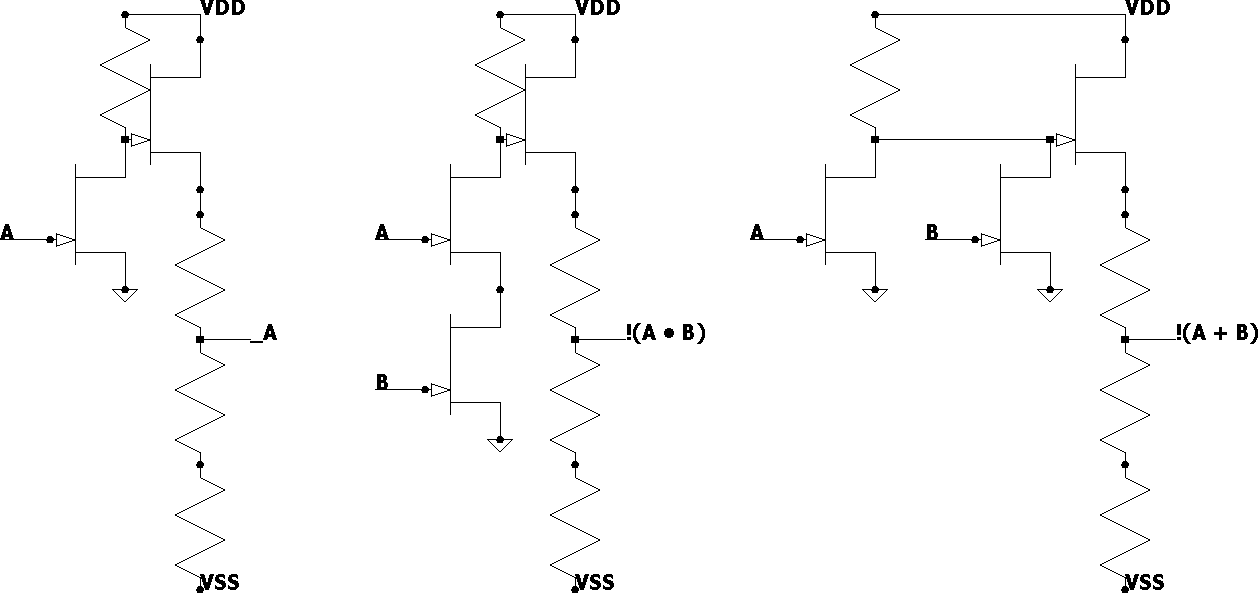
\includegraphics[width=1\linewidth]{Images/Inverter.pdf}
    \caption{Circuit diagrams of NOT, NAND, and NOR gates respectively}
    \label{fig:Inverter}
\end{figure}

The LTspice model of the JFET was used to create a logic primitive. This was extended to form more complex Logic Gates. Applying a voltage to the Gate of a JFET causes the depletion region to increase. This narrows the conducting channel increasing the resistance, which decreases the current that can pass through it. If the source of the JFET is connected to a voltage source through a resistor there will then be a change in voltage at the JFET's source when a voltage is applied to the Gate. This does not provide a large enough voltage swing between high and low and has implications for the fan out of the gate. Therefore, a voltage follower was used which works as a voltage level shifter and shifts the output voltage back to input levels of the logic gate (High: -0.8 V, Low: -3.6 V). These values were selected as they kept the output voltage from decaying or oscillating when used as inputs for subsequent gates whilst using standard resistor values.

The design of more complex gates follows on logically from this (Figure \ref{fig:Inverter}). To design the NOR gate a second JFET can be connected to the voltage follower in parallel with the first JFET which provides two inputs both with equal function. This means that if either JFET has a voltage applied, the output of the logic gate is the same. The NAND gate was developed using similar reasoning. If both inputs are required to be on to turn the output off, connecting two JFETs in series to the voltage follower will require that both JFETs are sinking current for the output to change. Condensed boolean gates are gates that have an entire Boolean expression compressed into a single gate in order to optimise the number of transistors used (Figure \ref{fig:Multigate}). For example, a NOR gate in which one input JFET is replaced by two JFETs in series to ground produces $\overline{AB + C}$ while saving two devices compared to the equivalent NAND/NOR composition. This is analogous to the use of complex gates in integrated-circuit logic design, where several Boolean operations are collapsed into a single transistor network to reduce device count.

\begin{figure}[t]
    \centering
    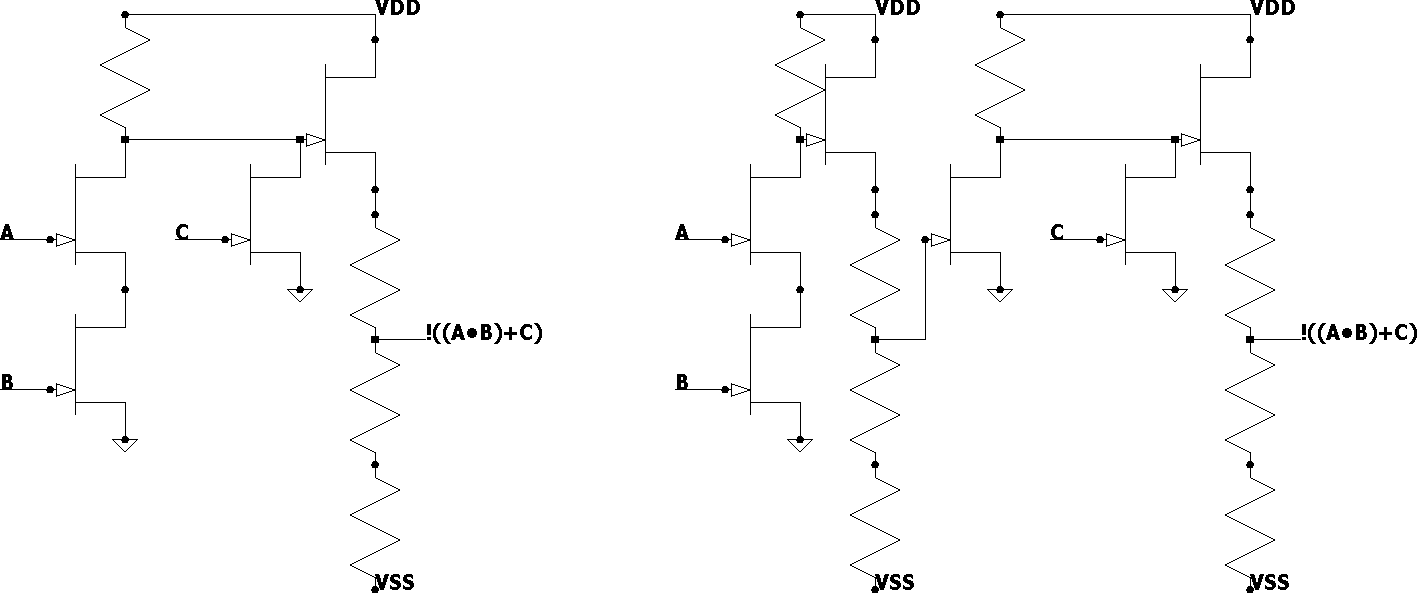
\includegraphics[width=1\linewidth]{Images/MultiGate.pdf}
    \caption{Circuit diagram of a condensed boolean gate (Left) and a combination of base gates (Right), illustrating the transistor reduction for the boolean equation (A AND B) NOR C}
    \label{fig:Multigate}
\end{figure}

The nominal electrical parameters used throughout this paper are summarised in Table~\ref{tab:rtl-params}. NAND and NOR gates were built in the lab and compared to the simulated devices, characterised from 1\,Hz up to a maximum of 1\,MHz; results are presented in Section~\ref{sec_results}.

\begin{table}[t]
\centering
\caption{Nominal SiC JFET RTL simulation parameters, as defined in \texttt{cpus/4004/config.py}.}
\label{tab:rtl-params}
\begin{tabular}{@{}lr@{}}
\toprule
Parameter & Value \\
\midrule
Positive supply $V_\text{POS}$ & $+24$\,V \\
Negative supply $V_\text{NEG}$ & $-20$\,V \\
Logic high & $-0.8$\,V \\
Logic low & $-3.6$\,V \\
Threshold (digital analyser) & $-2.5$\,V \\
Pull-up resistor $R_1$ (INV/NAND2/NOR2) & $50$\,k$\Omega$ \\
Voltage-follower upper $R_2$ & $1$\,k$\Omega$ \\
Voltage-follower lower $R_3$ & $4.5$\,k$\Omega$ \\
JFET gate--source / gate--drain $C_{gs0},\,C_{gd0}$ & $16.9$\,pF \\
Simulation temperature & $27$\,$^{\circ}$C \\
Target clock frequency & $100$\,kHz \\
\bottomrule
\end{tabular}
\end{table}

\subsection{CPU Design}\label{CPUDes}

\ifjxcdc
%---------------------- JXCDC compressed subsystem walk ----------------------
The Intel 4004 decomposes into six subsystems, each captured in LTspice and verified in isolation before integration: a 4-bit \emph{ALU} (Figure~\ref{fig:4004Architecture}) consisting of a 4-bit ripple-carry adder, accumulator and temporary registers, a separate incrementer for scratch-pad register updates, and a two-stage carry flag that breaks the write-back / read race between sum and carry; an \emph{instruction register and decoder} that demultiplexes the high 8 bits of each fetched word into a one-hot instruction line and AND-combines it with a micro-instruction step counter to drive subsystem control lines across three named phases ($A_{1,2,3}$, $M_{1,2}$, $X_{1,2,3}$); a \emph{program counter} with a dedicated 12-bit datapath to a 3-level subroutine \emph{stack}, since the four-bit shared bus cannot move 12 PC bits inside the three-clock execute window; a \emph{sixteen-register 4-bit scratch pad} with pair-mode and individual-word addressing modes; a 4-bit external \emph{bus} treated as a multi-input OR rather than tri-state because the JFET RTL voltage levels do not implement high-impedance cleanly; and a set of \emph{external pins} for data, four CM-RAM signals, CM-ROM, and SYNCH. Per-subsystem JFET counts are given in Table~\ref{tab:transistor-count}. Full transistor-level schematics for every subsystem, the carry-stage race-condition derivation, and the micro-instruction phase enumeration are given in the supplementary material.

\begin{figure}[t]
    \centering
    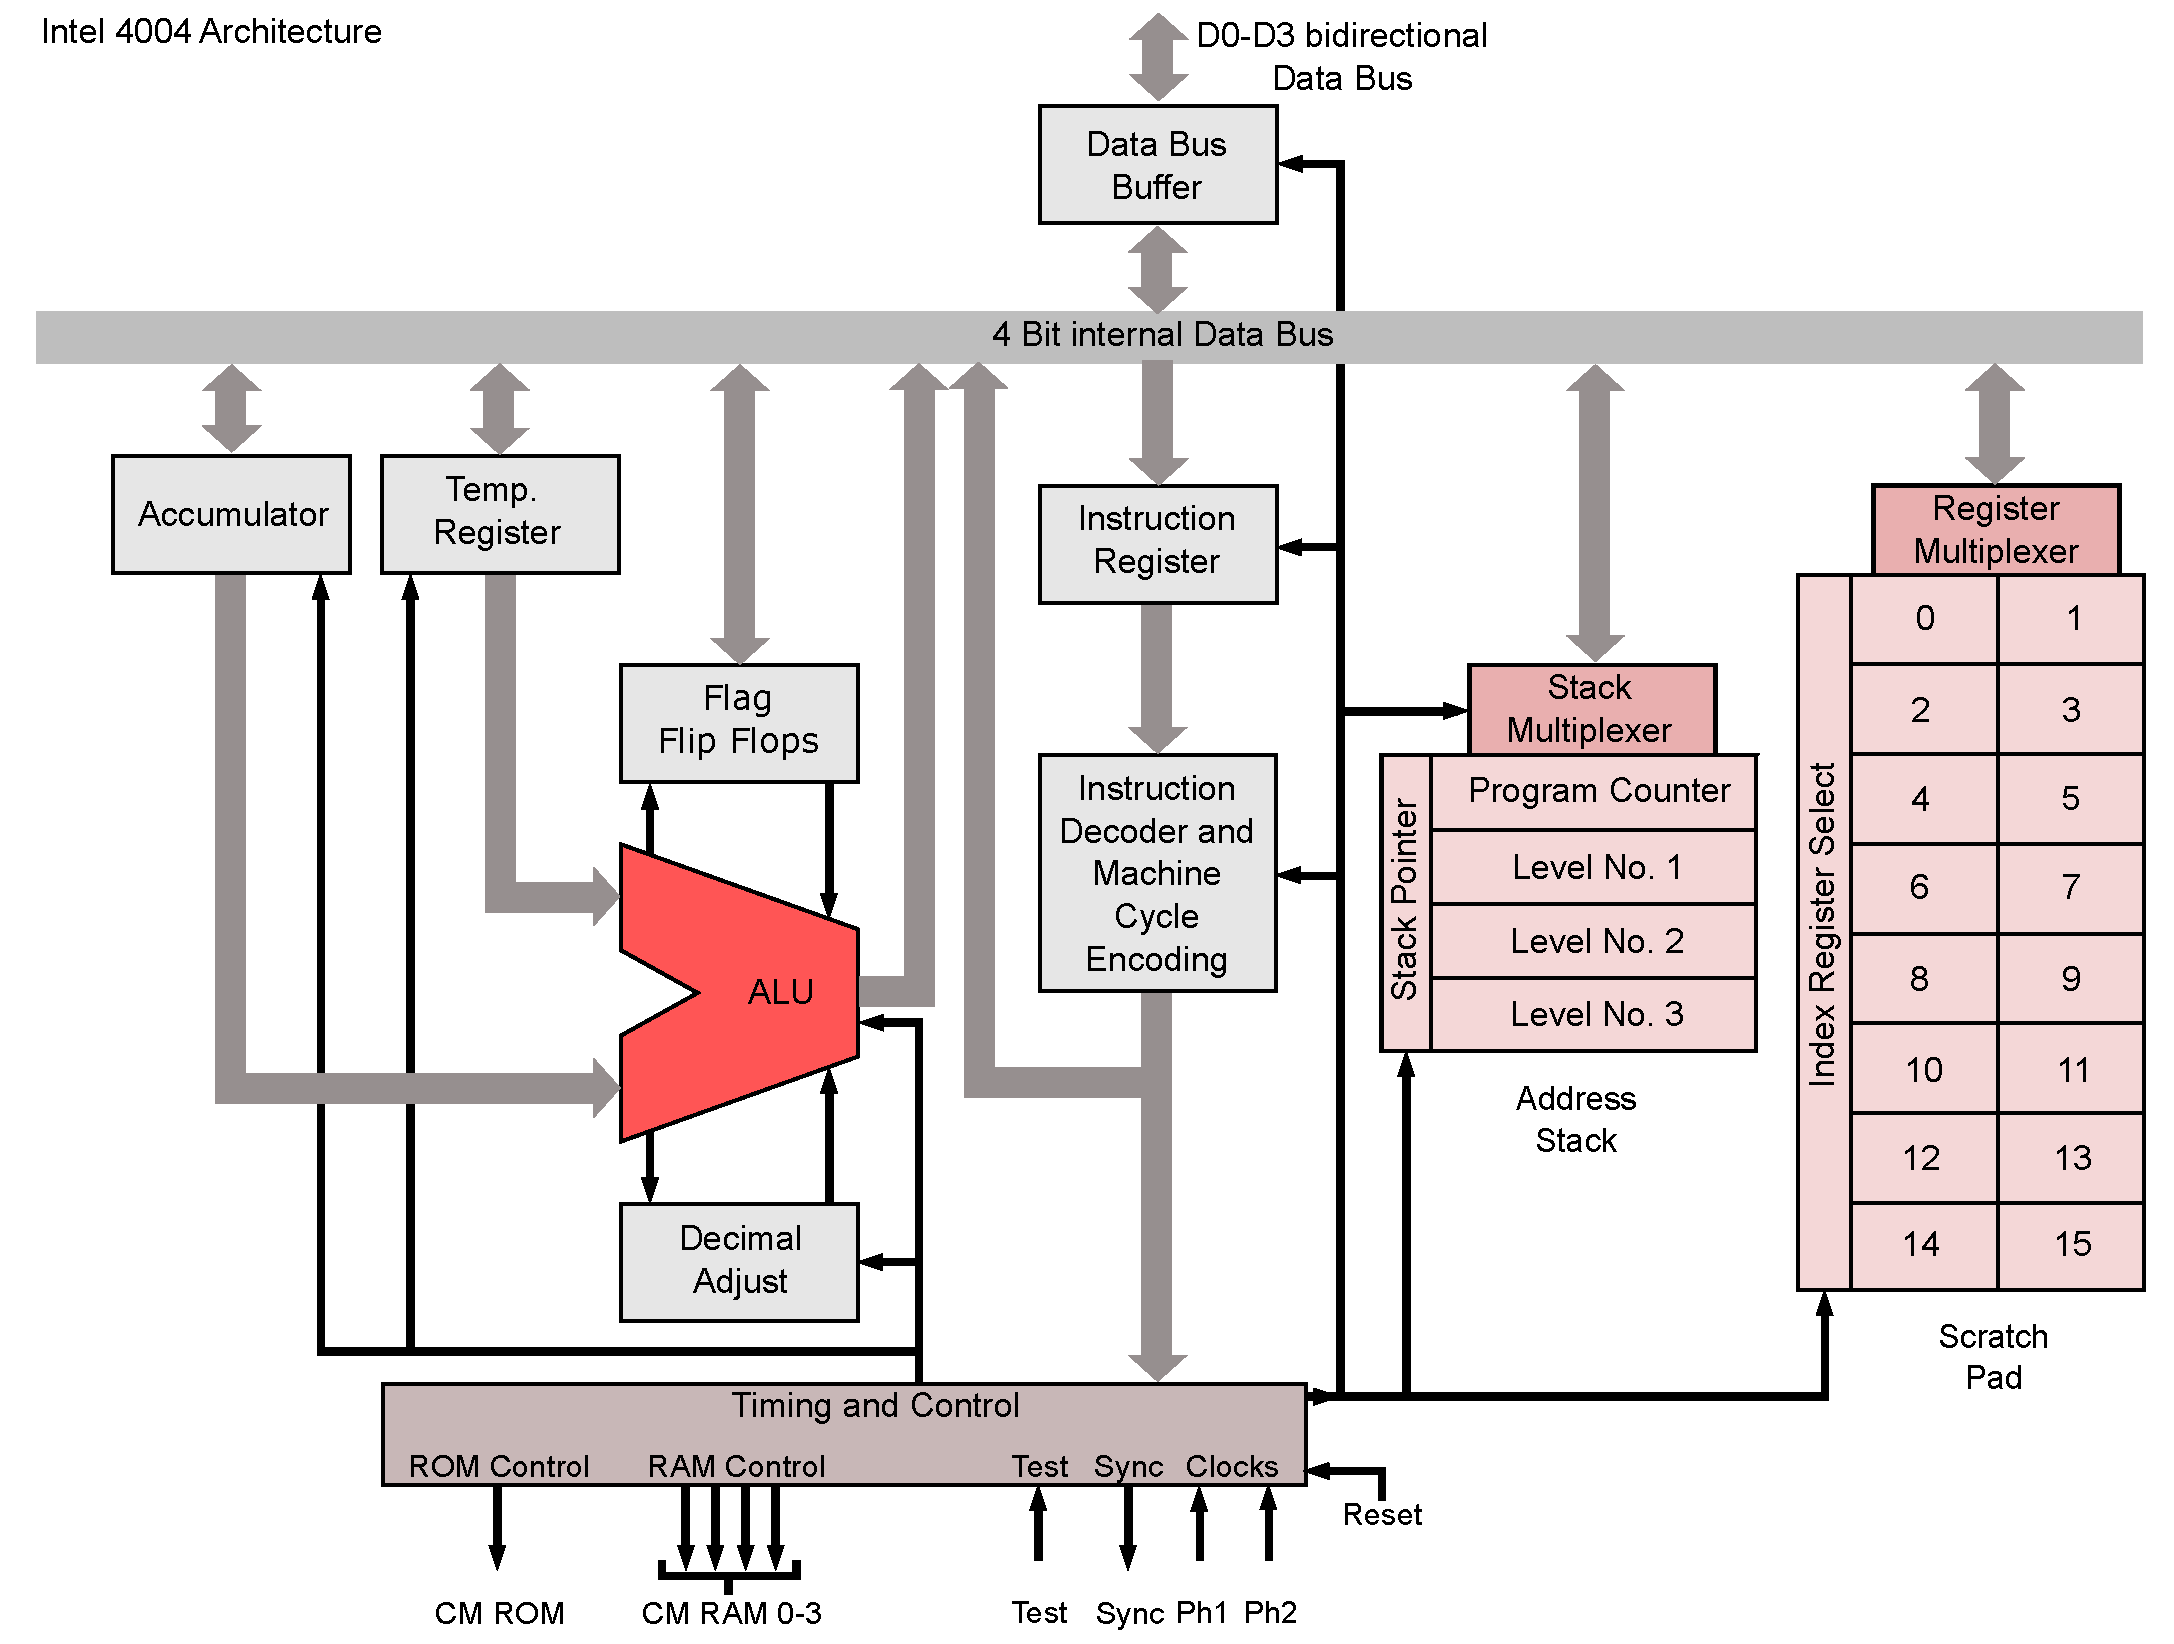
\includegraphics[width=1\linewidth]{Images/4004Architecture.pdf}
    \caption{Architecture of the Intel 4004 \cite{Archi} showing the layout of registers and connections between CPU sub-systems. Full transistor-level schematics for each subsystem are in the supplementary material.}
    \label{fig:4004Architecture}
\end{figure}

\else
%---------------------- Full subsystem walk (master) ----------------------
The Intel 4004 can be decomposed into several distinct sub-systems. The arithmetic logic unit (ALU), the instruction register and decoding, the stack and program counter (PC), the Scratch Pad, and the circuits related to the pins and interfacing with other external components. The specific instructions relating to each sub-system were evaluated in detail to precisely match the functionality of the original Intel 4004.

\subsubsection{ALU}
From the architecture diagram (Figure \ref{fig:4004Architecture}) it can be seen that the ALU (Figure \ref{ALUDiag}) has two 4-bit registers connected to it, the Accumulator (Acc) and the Temporary (Temp) register. From the instruction set it can be seen that the ALU consists only of a 4-bit adder. The contents of the accumulator can also be shifted to the left or right by one bit, however it also includes the carry flag in this shift operation. For example, shifting right would place the least significant bit of the accumulator into the carry and what was in the carry into the most significant bit of the accumulator. Based on the instruction set it can be deduced that there is no inverter on the accumulator and that for subtraction and the other inversion instructions, for example complement accumulator (CMA), there must be an inverter between the temporary register and its connections to the bus and adder. CMA is then accomplished by transferring the value from the Accumulator to the Temp register, inverting the Temp register and transferring this inverted value back to the Accumulator. The carry flag also needs to be able to be inverted. There is a separate incrementer circuit which adds one to the temporary register. This is because the instruction Increment (INC), increments the value stored in a specific Scratch Pad register without effecting the accumulator or the carry flag of the ALU. There is not enough time in the execute portion of the instruction cycle for the accumulator value to be moved to some intermediate location to be moved back after the increment instruction is completed. This means that there has to be a separate circuit for incrementing Scratch Pad registers.

\begin{figure}[t]
    \centering
    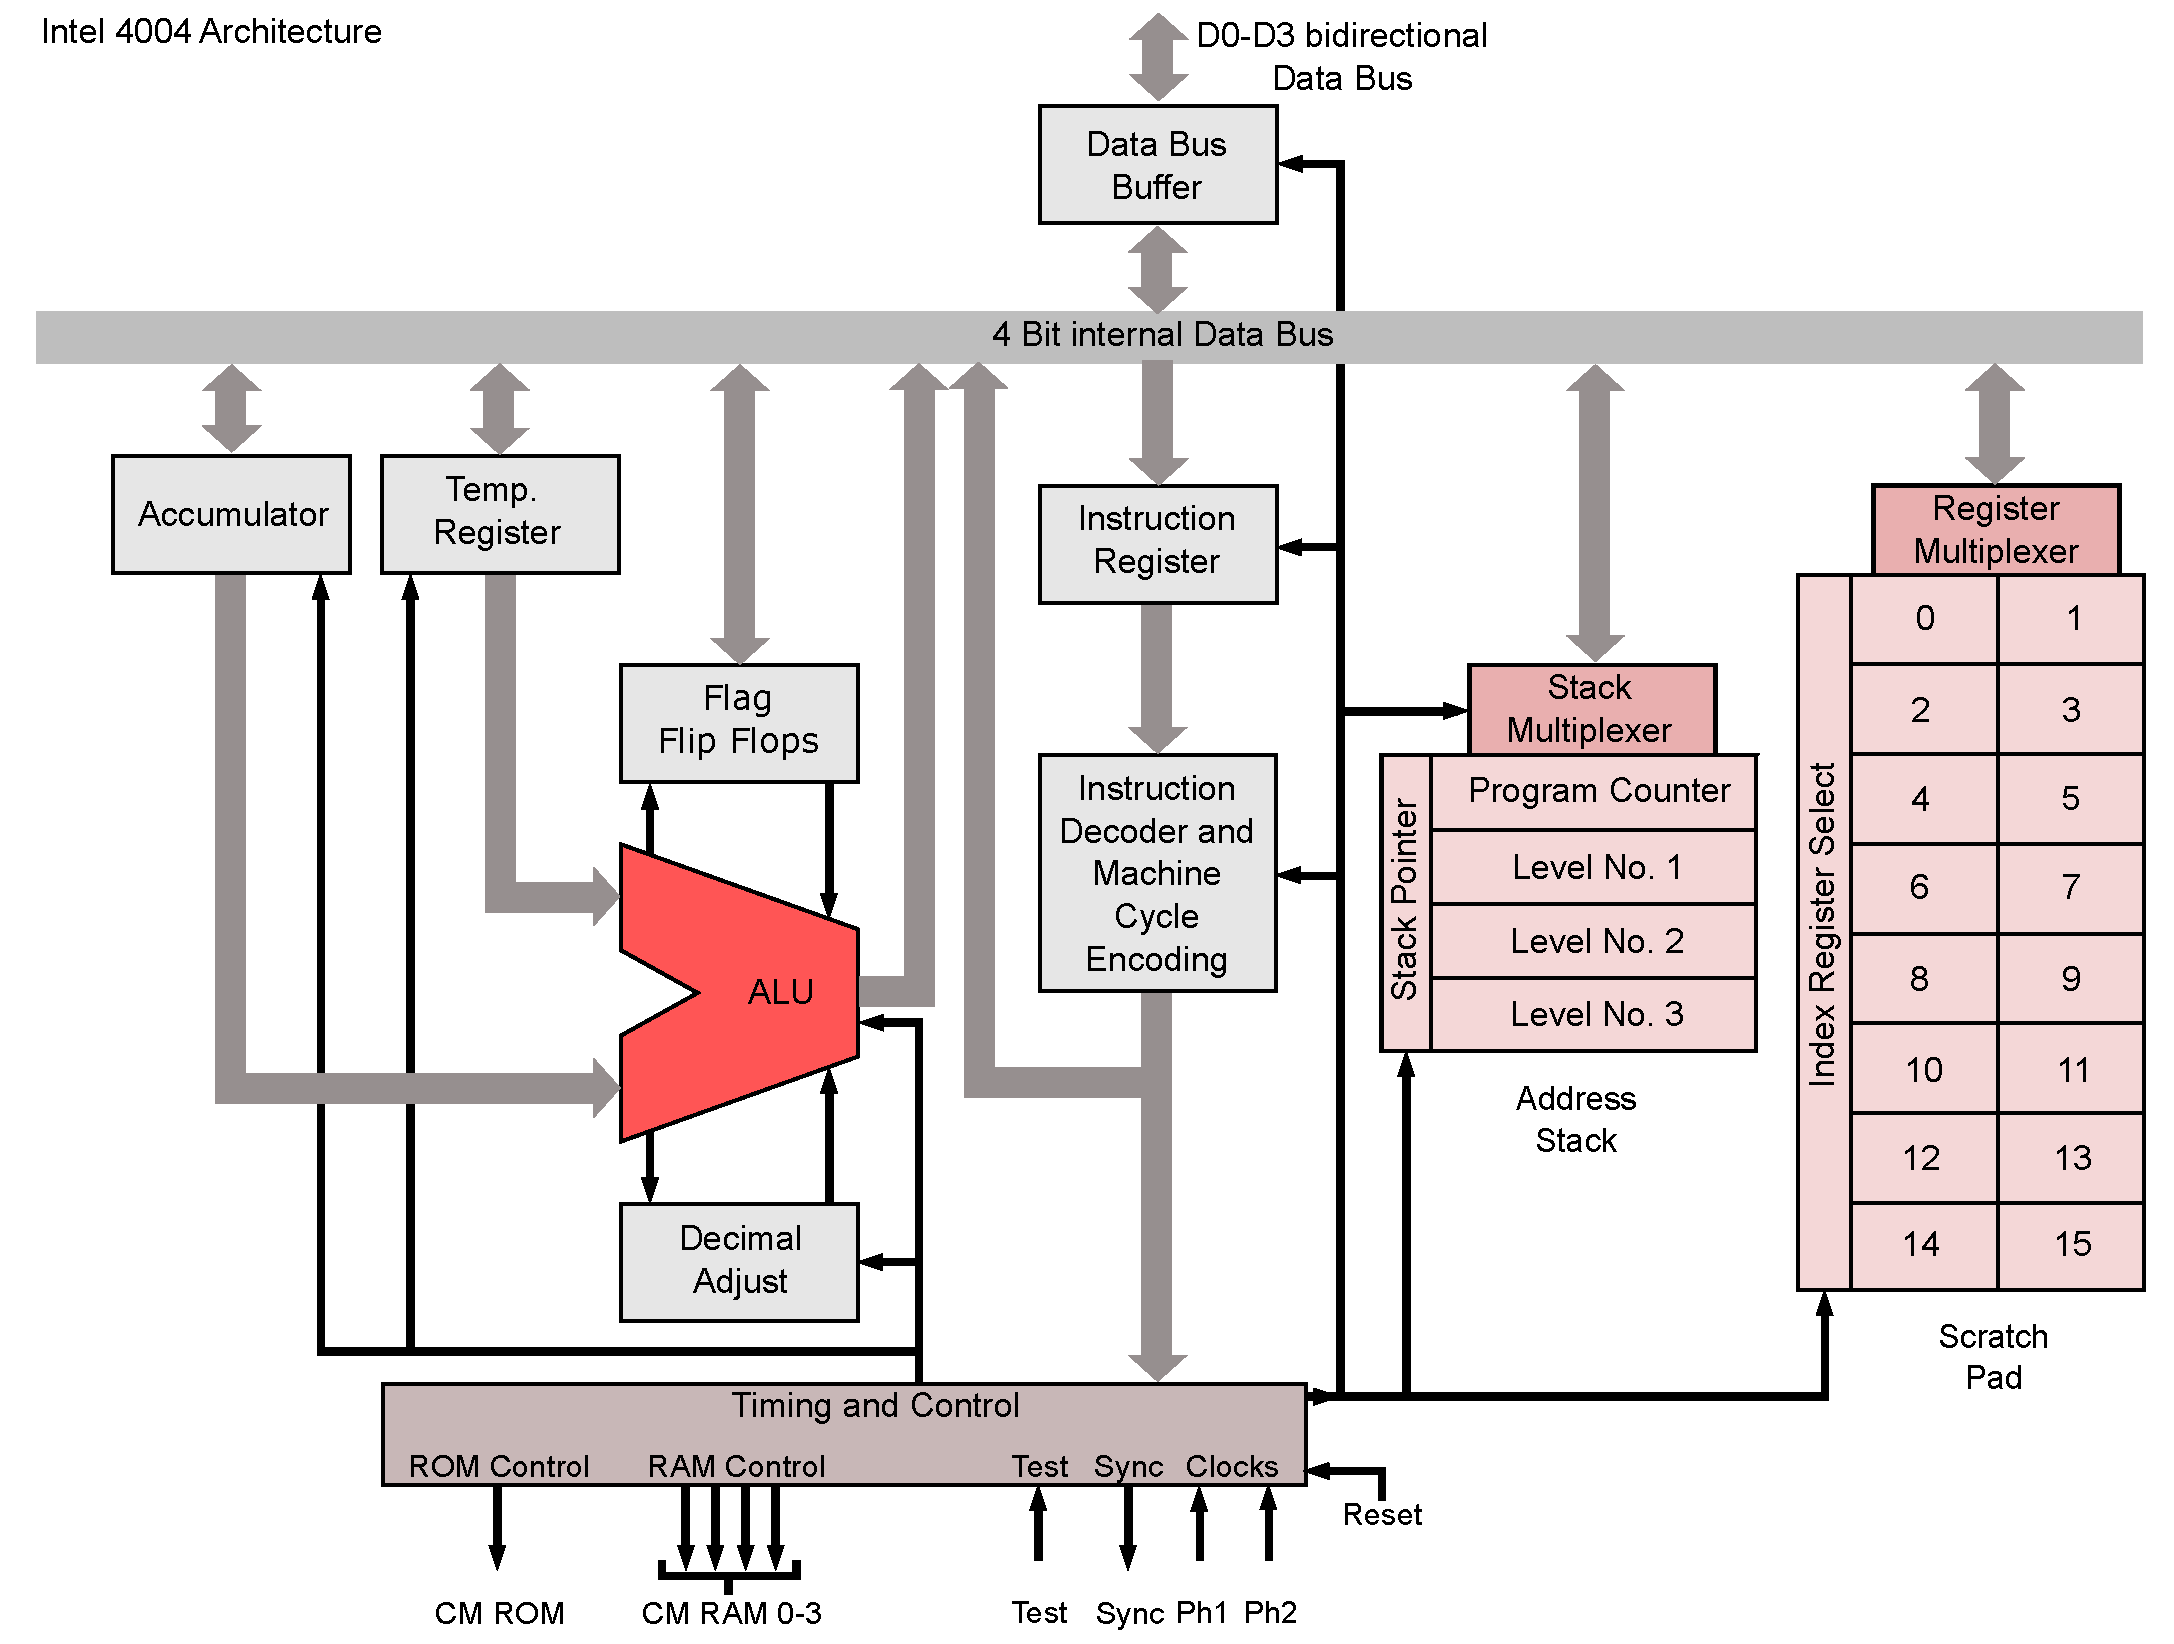
\includegraphics[width=1\linewidth]{Images/4004Architecture.pdf}
    \caption{Architecture of the Intel 4004 \cite{Archi} showing the layout of registers and connections between CPU sub-systems}
    \label{fig:4004Architecture}
\end{figure}

\begin{figure}[b]
  \centering
  \includegraphics[width=\linewidth]{Images/ALUAnnotated.pdf}
  \caption{Circuit diagram for the Arithmetic and Logic Unit with colour-coded sub-circuits}
  \label{ALUDiag}
\end{figure}

A two-stage carry flag is required because the carry and accumulator do not latch their new values simultaneously, producing a race condition between the sum write-back and the carry update. The first flip-flop captures the new carry without affecting the adder input, and the second stage is loaded from the first once the accumulator has been written. The full derivation is given in Supplementary Note S1.

\subsubsection{Instructions}

\begin{figure}[b]
  \centering
  \includegraphics[width=1\linewidth]{Images/InstructionRegisterAnnotated.pdf}
  \caption{Circuit diagram for the Instruction Register with colour-coded sub-circuits}
  \label{fig:InstructionReg}
\end{figure}

The instruction register of the 4004 is 16-bits wide (Figure \ref{fig:InstructionReg}). Instructions are one or two eight-bit words; the most significant four bits are an opcode and the remaining bits encode an operand or, in a small number of cases, an opcode discriminator (for instance, the LSB of the lower nibble distinguishes FIN from JIN). The high eight bits are de-multiplexed to produce a one-hot instruction-selected line that, when AND-ed with the current micro-instruction step counter (Figure \ref{fig:StepCounter}), generates each of the per-step control-line activations that constitute a micro-instruction (Figure \ref{MicroInstructionExp}). Each instruction is executed across three named phases --- address ($A_{1,2,3}$), memory ($M_{1,2}$) and execute ($X_{1,2,3}$) --- under which the CPU drives the address onto the four-bit external bus in the order required by the 4001 ROM and the 4002 RAM, captures eight bits of returned data into the instruction register, and finally asserts the subsystem control lines required to complete the operation. Two-word instructions are handled by a single toggle flip-flop on the CPU that re-enters the lower-word load path on the next fetch cycle. The full phase-by-phase enumeration, including the ROM-side handshake, is given in Supplementary Note S2.

\begin{figure}[t]
  \centering
  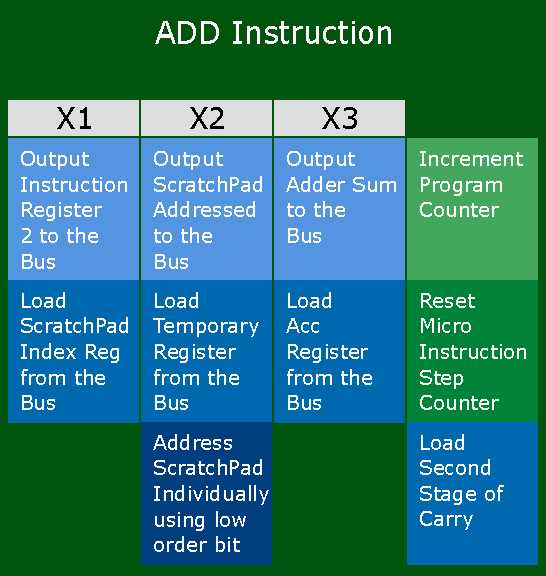
\includegraphics[height = 4.8cm, width = 4.8cm]{Images/MicroInstructionExp.pdf}
  \caption{Diagram showing the control lines that need to be activated per step to execute the ADD instruction}
  \label{MicroInstructionExp}
\end{figure}

\begin{figure}[b]
    \centering
    
\includegraphics[width=1\linewidth]{Images/Step Counter.pdf}
    \caption{Circuit diagram for the Micro-Instruction step counter, composed of a series of 1-bit registers}
    \label{fig:StepCounter}
\end{figure}

\subsubsection{Program Counter and Stack}
The Program Counter (PC) (Figure \ref{fig:ProgramCounter}) consists of a 12-bit register and an incrementing circuit. The PC also needs to be able to write values to and from the Bus. The conditional jump (JCN) instruction indicates that each 4-bits in the PC need to be individually controlled as the high order 4-bits are not changed when JCN is performed. The limit of three micro-instruction steps for executing instructions means that the stack (Figure \ref{fig:Stack}) has to have a direct connection to the PC as all 12-bits need to be written, along with additional steps related to the stack level control, within three clock pulses. This is not possible with the 4-bit bus unless the PC and Stack have a direct connection. The stack is three layers deep and needs to keep track of which level it is on. This is done using a shift register which is able to be shifted up and down to select each level. The output of each register of the stack is fed into an AND gate along with the level control line that corresponds to it so that the register only outputs when its level is selected and the "Output Stack" control line is enabled.

\begin{figure}[t]
    \centering
    \includegraphics[width=1\linewidth]{Images/ProgramCounterAnnotated.pdf}
    \caption{Circuit diagram for the Program Counter with colour-coded sub-circuits}
    \label{fig:ProgramCounter}
\end{figure}
\begin{figure}[b]
    \centering
    \includegraphics[width=1\linewidth]{Images/StackAnnotated.pdf}
    \caption{Circuit diagram for the Stack with colour-coded sub-circuits}
    \label{fig:Stack}
\end{figure}

\subsubsection{Scratch Pad}
The 4004 has sixteen 4-bit registers it can use as general purpose memory. This is so that it is able to perform basic functions without the need for any external RAM chips. It is known as the Scratch Pad (Figure \ref{fig:Scratch Pad}). Each Scratch Pad location can be addressed individually or as a pair of registers for storing 8-bit values. The Scratch Pad has its own address register. When the Scratch Pad is in pair-mode the highest order 3-bits of the address are used to select a register pair. The instruction then places the value of each register of the pair onto the bus sequentially. When the Scratch Pad is being individually addressed the full address is looked at and the control signal for the correct register is generated. This is done with a separate "Scratch Pad Register Select" control line which is fed into an AND gate with the least significant bit from the Scratch Pad address register. This then generates a "Word Select" line which in turn activates either the first or the second word of the specified pair of registers.

\begin{figure}[t]
    \centering
    \includegraphics[width=1\linewidth]{Images/ScratchPadAnnotated.pdf}
    \caption{Circuit diagram for the Scratch Pad with colour-coded sub-circuits}
    \label{fig:Scratch Pad}
\end{figure}

\subsubsection{Bus}
The internal data bus on a tri-state PMOS 4004 carries three states (logic high, logic low, and high impedance). The voltage-follower output stage of the SiC JFET RTL primitives used here does not implement a clean high-impedance state, so each producer of the four-bit internal bus is instead connected through what is effectively a multi-input OR: if any enabled producer asserts logic high, the bus reads logic high, otherwise it reads logic low. Bus contention is avoided at the micro-instruction-control level rather than at the electrical level -- only the intended producer is enabled by the step counter during each micro-instruction phase, and the OR-style combining is used to obtain stable RTL voltage levels rather than the high-impedance behaviour of the original. The connection from the bus to each circuit's input is conventional, since these connections all terminate at JFET gates and so do not exhibit the same voltage-combining problem at the producing side. This deviation preserves the software-visible value placed on the modelled internal data bus in the tested programs (Section~\ref{sec_results}), but it is not pin-level equivalent to the original 4004 external bus protocol; see the definition of ``4004-compatible'' at the start of Section~\ref{theory}.

\subsubsection{Pins and Communication}
The 4004 has a number of pins used to interface with external components (Figure \ref{fig:Pins}). There are four data pins which are used to transfer opcodes and data between the CPU and the external bus ($D_{0,1,2,3}$). There are four CM-RAM pins which are used to address the RAM chips ($CM-RAM0,1,2,3$). When the designate command line (DCL) instruction is executed the value that is in the accumulator is loaded into the CM-RAM register. These pins are "1 Hot" due to the fact that each RAM chip only has one CM-RAM input pin. However, the user is able to put an external de-multiplexer in between the CM-RAM pins and the input of the RAM chip to allow for the full address space to be used rather than just the maximum of four chips as default. The CM-ROM pin is used to communicate with the ROM and the RAM. This pin will go high at specific points in the instruction cycle to indicate various things such as a ROM/RAM instruction. Finally the SYNCH pin which is used to synchronise the operations of all chips in a larger circuit.

\begin{figure}
    \centering
    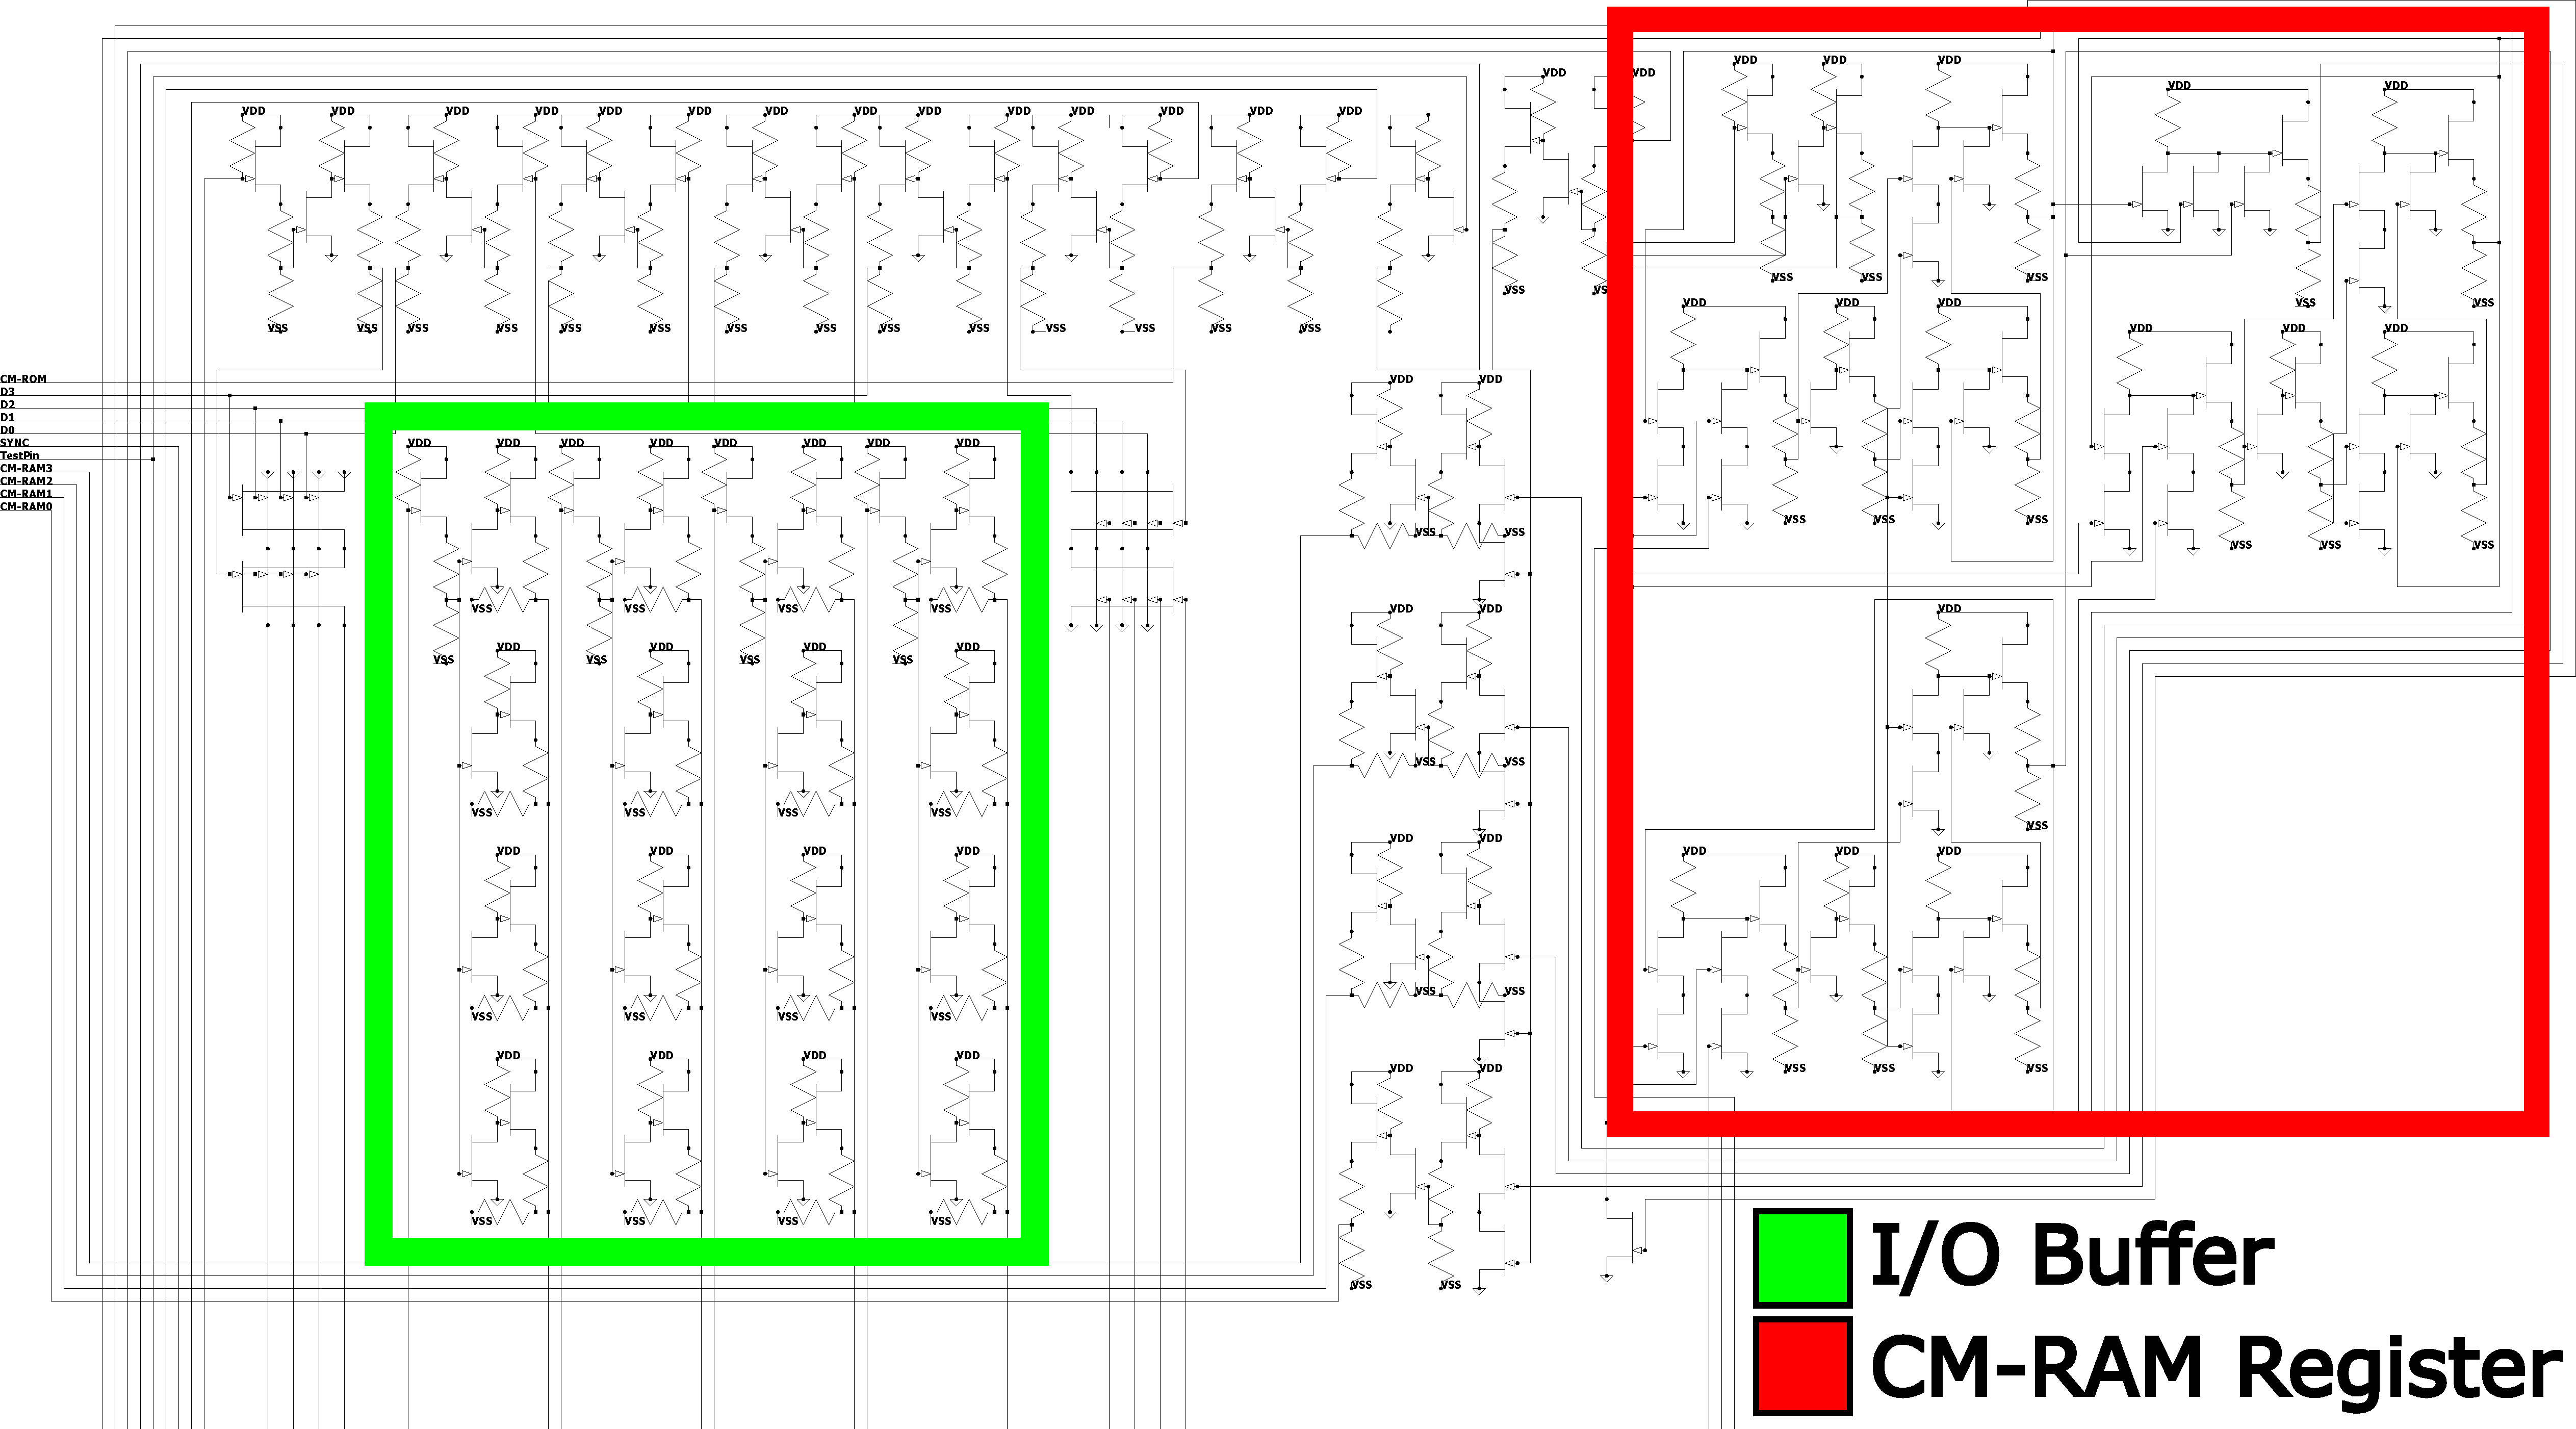
\includegraphics[width=1\linewidth]{Images/PinsAnnotated.pdf}
    \caption{Circuit diagram for the pins and associated logic with colour-coded sub-circuits}
    \label{fig:Pins}
\end{figure}
\fi
%---------------------- end CPU Design conditional ----------------------

\section{Method}\label{method}
Validation proceeded hierarchically: primitive gates were first checked in LTspice, then composed into sequential subcircuits and CPU subsystems before full-processor integration. The first sequential subcircuit was the 1-bit synchronous D-type flip-flop. The synchronous part of this simply means that it only latches the D value in on the clock pulse. First the flip-flop was built using discrete logic gates, however, it was noticed that some gates could be reduced using condensed boolean gates as described in the logic primitives section (Section \ref{primitives}). This was done until the circuit could not be condensed any further due to race conditions and the path for individual signals becoming unbalanced compared to other paths through the circuit. This unbalancing occurred due to the layout of the logic circuit for a D-type flip-flop. The output is taken from a pair of cross-connected gates meaning that if one gate was reached by the signal significantly before the other gate, the output would not latch correctly (Figure \ref{DFlopLogi}). D flip-flops were used for storage in this CPU as 6-transistor (6T) static RAM (SRAM) and 1-transistor (1T) dynamic RAM (DRAM) proved challenging to implement. There are 146 bits of storage in the 4004; with the current 15-JFET D flip-flop, this accounts for 2190 of the processor's transistors. The full per-subsystem JFET budget of the implementation is given in Table~\ref{tab:transistor-count}; the scratch pad and stack together consume \JFETCountScratch{} and \JFETCountStack{} JFETs respectively, dominating the total of \TotalJFETCount{}. This total is regenerated from the released schematic metadata using \texttt{tools/count\_transistors.py}, which walks the \texttt{SYMBOL njf} declarations in every component file referenced by the CPU configuration. The count differs slightly from the preliminary hand count of 5328 in earlier reports of this work, which understated the scratch-pad and stack subsystems. Development of 1T DRAM would, by inspection, reduce the total transistor count by roughly 2000 (excluding any RAM refresh circuitry), making storage technology the highest-leverage target for further reduction.

% Auto-generated by tools/count_transistors.py -- do not edit by hand.
\begin{table}[t]
\centering
\caption{Transistor count of the SiC JFET 4004-compatible processor, per subsystem at full capacity (all sixteen scratch-pad registers and three stack levels included). Numbers are derived directly from the LTspice schematics referenced by \texttt{cpus/4004/config.py}; re-running \texttt{tools/count\_transistors.py} regenerates this table from the current schematic state.}
\label{tab:transistor-count}
\begin{tabular}{@{}lrrr@{}}
\toprule
Subsystem & JFETs & \% of total & Resistors \\
\midrule
Arithmetic logic unit & 566 & 10.2\% & 504 \\
Instruction register & 680 & 12.3\% & 642 \\
Micro-instruction decoder & 877 & 15.8\% & 675 \\
Control logic & 28 & 0.5\% & 24 \\
External pins and bus & 140 & 2.5\% & 159 \\
Program counter & 503 & 9.1\% & 429 \\
Step counter & 363 & 6.6\% & 351 \\
Scratch pad ($16\times 4$-bit) & 1563 & 28.2\% & 1230 \\
Subroutine stack (3-level) & 817 & 14.8\% & 693 \\
\midrule
\textbf{Total} & \textbf{5537} & \textbf{100.0\%} & \textbf{4707} \\
\bottomrule
\end{tabular}
\end{table}

Each sub-system of the CPU was built separately at first in order to decrease simulation times. The system was tested using the following method. Each control line was connected to a voltage source utilising a Piecewise linear (PWL) file. A PWL file is a type of file used by LTspice which specifies the voltage at specific time points. Each control line was listed in a spreadsheet along with register values if appropriate. The necessary voltage level for each control line was then plotted on a timeline to "program" the circuit to perform operations. The PWL files were then generated using Matlab from the list of times the control line needed to be high. The final state of the sub-system could then be compared to the expected state calculated from the spreadsheet. Once each sub-system had been verified as correctly functioning they were assembled into the full CPU by means of a Python script which collated each sub-system and renamed any duplicated component names. This was then tested by connecting the bus to voltage sources and emulating the ROM by feeding it data when it expected to receive data from the ROM. This approach was sufficient for deterministic subsystem tests, but could not validate programs whose control flow depended on CPU-computed state, since every bit returned to the CPU had to be hard-coded beforehand.

\begin{figure}
    \centering
    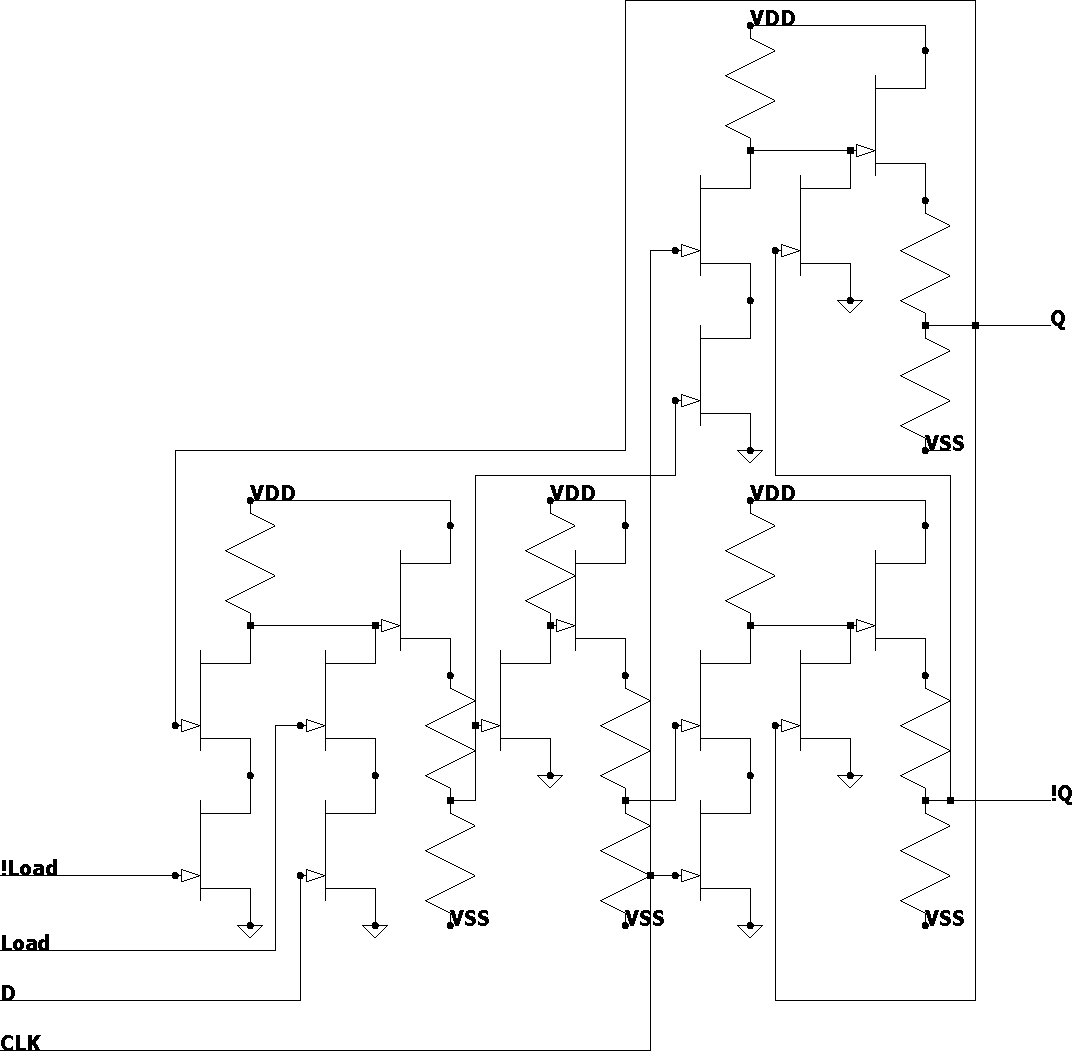
\includegraphics[width = 1\linewidth]{Images/DFlipFlop.pdf}
    \caption{Circuit diagram for synchronous D-type flip-flop with transistor reductions using combined boolean logic gates}
    \label{DFlopLogi}
\end{figure}

\ifjxcdc\else
\subsection{ROM}
In order to fully test the capabilities of this CPU it was decided that a ROM needed to be designed and built (Figure \ref{ROMDIAGRAM}). The 4001 functions in a similar way to the 4004. It uses a micro-instruction counter to see where it is in the instruction cycle and also has an instruction register which is used for some ROM specific instructions. The ROM receives an address from the CPU at times $A_1$ and $A_2$. It then receives a chip select address at time $A_3$, which determines which of the 4001 chips is being addressed, along with CM-ROM going high. Each 4001 has a specific identity which is hard-wired during production. If the value that is wired into the 4001 matches the address received at $A_3$ the 4001 then outputs the values stored at the address received from $A_{1,2}$ during $M_1$ and $M_2$ otherwise it is deactivated until the next fetch cycle. If a ROM/RAM instruction is detected by the ROM, the instruction register is loaded from the external bus during $X_1$. The ROM has two instructions as implemented in this paper, write ROM port (WRR) and read ROM port (RDR) which are used to read and write to the I/O pins on the ROM chip. This is performed during $X_2$ unless no instruction was received during $X_1$ in which case the execution cycle is reset ready for the next address to be received. Storage in the ROM was implemented using a voltage source linked to a PWL file for each bit of every address. When the ROM is addressed the value defined by the PWL file for that address is sent out onto the bus. This was done so that each bit would have a specific PWL file which could be written to, allowing for the ROM to be programmed.

\begin{figure}
    \centering
    \includegraphics[width=1\linewidth]{Images/ROM.pdf}
    \caption{Circuit diagram for computational part of Intel 4001 with colour-coded sub-systems}
    \label{ROMDIAGRAM}
\end{figure}
\fi

\subsection{Assembler}
An assembler converts the mnemonics of the instructions from text to binary and converts the operands from hexadecimal or decimal to binary. Thus \texttt{FIM 1 0 11} is converted to \texttt{0010 0010 0000 1011}. The assembler is a two-pass implementation. The first pass walks the source text and records, for each label, the ROM byte address at which the next instruction will be emitted, advancing a running address counter by one byte per single-word instruction and by two bytes per two-word instruction (\texttt{JCN}, \texttt{FIM}, \texttt{JUN}, \texttt{JMS}, \texttt{ISZ}). The second pass emits the byte stream, with each label reference resolved to the recorded 12-bit ROM byte address rather than to a source-text line number. The assembled program is written to a \texttt{.bin} file -- one 8-bit ROM word per line, in ROM-address order -- and to a parallel \texttt{.hex} file. The assembler is written in Python.

\subsection{PWL File Generation}
The \texttt{.bin} file is used by another Python script to generate the PWL files that populate the voltage sources inside the 4001-style ROM model. Each PWL file encodes the fixed contents of a single ROM bit cell -- either a constant logical high ($-0.8$~V) or a constant logical low ($-3.6$~V) -- and is named \texttt{0.txt}, \texttt{1.txt}, $\ldots$ in ROM-bit order. Address decoding inside the ROM model selects the addressed byte during the simulated $M_1$/$M_2$ phases, so branch and subroutine behaviour during simulation is determined by the CPU state and the ROM address path rather than by an externally scripted bus trace; the PWLs do not encode a precomputed execution trace.

\subsection{Testing and Benchmarking}
With a full 4001 and a full 4004 modelled in LTspice, complete programs can be run and their state compared, instruction by instruction, against an independent Python reference emulator (\texttt{tools/rom\_emulator.py} in the repository). The reference emulator implements the documented 4004 ISA, including the carry rules for ADD/SUB, the rotate-through-carry semantics of RAL/RAR, and the three-level stack handling of JMS/BBL. Two test programs are run: the bitwise AND subroutine from the MCS-4 programming manual~\cite{Intel1973MCS4} (a 30-byte routine that exercises XCH, RAL/RAR, ADD, JCN and JMS/BBL --- Figure~\ref{fig:11AND6}) and a 16-bit floating-point multiplication whose execution trace covers 451 dynamically executed instructions and exercises the full ALU through a deeper subroutine call tree. For each program the LTspice CPU is allowed to settle past its power-up transients, the Python emulator is synced to the LTspice register state at a documented sync point, and forward execution from that point compares $(\mathrm{ACC}, \mathrm{CY}, R_0, \ldots, R_{15})$ at every instruction boundary. The headline pass/fail counts reported in Table~\ref{tab:results-summary} use \texttt{--resync never}: any cascading divergence after the first mismatch is exposed rather than papered over. A separate \texttt{--resync on-divergence} diagnostic mode re-aligns the emulator to the LTspice state after each mismatch and is used only to localise independent local errors; it is not used to claim end-to-end program correctness. Section~\ref{sec_results} presents the resulting per-program diff summaries.

\begin{figure}[t]
    \centering
    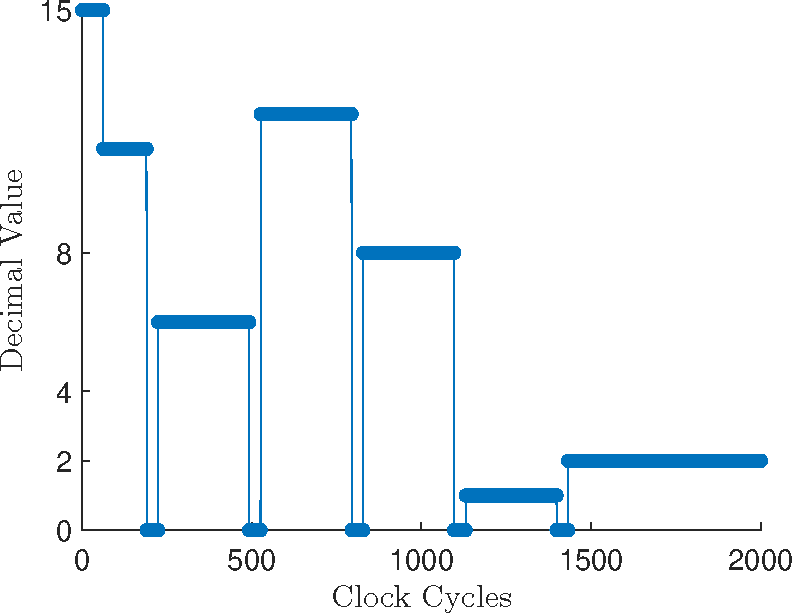
\includegraphics[height=4cm]{Images/11AND6.pdf}
    \caption{Figure showing the decimal value in Scratch Pad Register 0 for the operation 11 \& 6. This illustrates the first input (11) being shifted left 4 times to compare the highest order bit to the second input (6) with the final result of 2 being loaded in just before 1500 clock cycles}
    \label{fig:11AND6}
\end{figure}

\subsubsection{Waveform Analyser and Reference Emulator}
The LTspice \texttt{.raw} file is parsed directly by a Python tool (\texttt{tools/trace\_synced.py}) which thresholds the per-bit register node voltages at $-2.5$\,V to recover digital values, samples them at 95\% through each \texttt{micro1} phase (after the IR and accumulator have settled), and emits one nibble per register per instruction boundary. A 4004 ISA-level reference emulator written in Python (\texttt{tools/rom\_emulator.py}) is run in lockstep on the same machine code. Implementation quirks of the original 4004 --- the incrementer not affecting the accumulator, the LSB convention for FIN/JIN, the rotate-through-carry semantics --- were validated against an online JavaScript emulator~\cite{Emu} during development and against the contemporary MCS-4 manual~\cite{Intel1973MCS4}.

\subsection{Experimental Validation of Simulation Models}
Physical validation was performed on NAND and NOR primitives implemented using the available SiC JFET integrated circuit (IC) and a copper circuit board with through-hole components. These were connected to a power supply, a function generator, and an oscilloscope. They were then tested at a range of frequencies from 1 Hz to 1 MHz. The data from this experiment was then used to characterise the gates. The inputs from the function generator were taken and a Matlab script was written to convert these into a PWL file which could then be used as the inputs for the simulated gates to get an exact comparison between experimental and theoretical.

\ifjxcdc\else
\begin{figure}
\centering
\subcaptionbox{Significand which is calculated to be 166 in decimal\label{fig:sig}}
{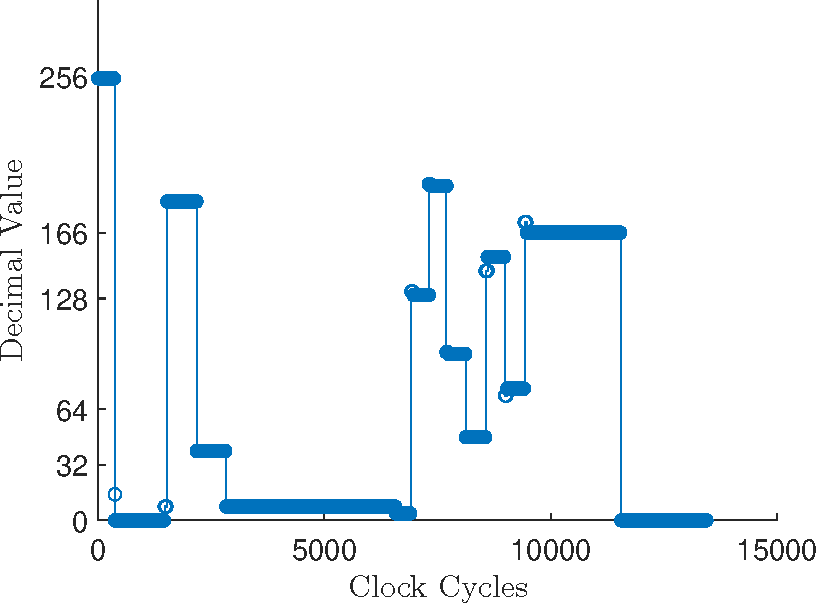
\includegraphics[width=0.49\linewidth]{Images/Mult.pdf}}
\subcaptionbox{Exponent which is calculated to be 65 in decimal\label{fig:exp}}
{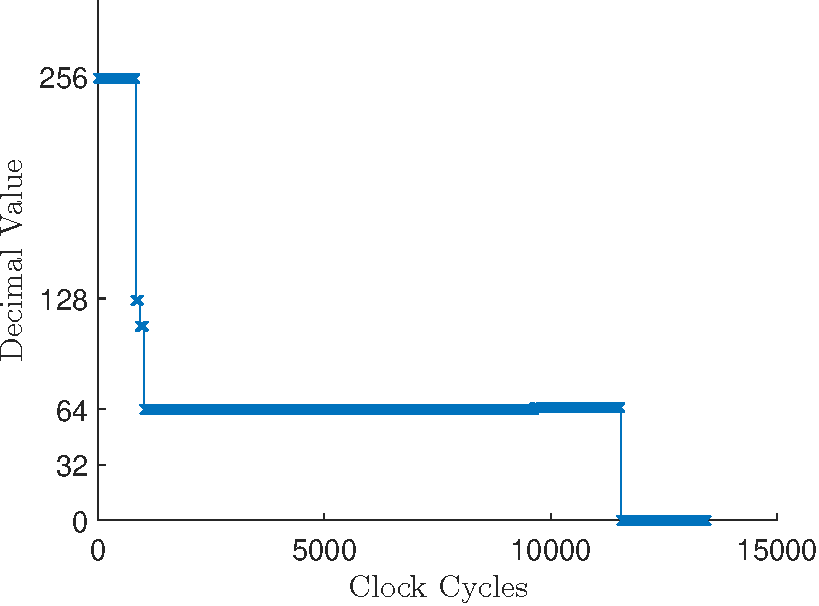
\includegraphics[width=0.49\linewidth]{Images/Mult2.pdf}}
\caption{The waveforms of the registers during the computation of the product of $1.4375 \times 3.60937$. Plots \ref{fig:sig} and \ref{fig:exp} show the values of the significand and exponent respectively during the operation}\label{fig:product}
\end{figure}
\fi

\section{Results and Discussion}\label{sec_results}

Table~\ref{tab:results-summary} collects the headline results of the work. Each row is detailed in the subsections that follow, and the limitations of each claim --- in particular the legacy nature of the NAND/NOR measurements and the room-temperature device model --- are discussed in Section~\ref{sec:limitations}.

\begin{table}[t]
\centering
\caption{Program-level LTspice/emulator co-validation. The compared state vector is $(\mathrm{ACC}, \mathrm{CY}, R_0, \ldots, R_{15})$. The headline pass/fail counts are computed without resynchronisation after the documented initial sync point; a separate resync-on-divergence mode (Section~\ref{method}) is used only for diagnostic localisation and is not used for the values reported here. ``Boundaries'' is the number of instruction boundaries compared after the sync point; ``mismatches'' is the number of those boundaries at which any element of the compared state vector differed between the LTspice CPU and the Python reference emulator.}
\label{tab:results-summary}
\begin{tabular}{@{}lrrrl@{}}
\toprule
Program & Bytes & Dyn.\ instr. & Boundaries / Mismatches & Final result \\
\midrule
AND subroutine    & 30 & \TraceCyclesBitwiseAND    & \TraceCyclesBitwiseAND\,/\,\TraceDivergencesBitwiseAND    & $R_0 = \texttt{0010}$ \\
FP multiplication & 51 & \TraceCyclesFloatingPoint & \TraceCyclesFloatingPoint\,/\,\TraceDivergencesFloatingPoint & $5.1875$ \\
\bottomrule
\end{tabular}
\end{table}

\noindent The primitive-gate physical evidence reported separately in Section~\ref{sec_results} below covers the NAND and NOR primitives only and supports the gate-level LTspice model rather than the full processor.

\subsection{Program Testing}
\subsubsection{AND Subroutine}
\ifjxcdc
The AND subroutine from the MCS-4 programming manual was run on the CPU and its register state compared to the Python emulator. Figure~\ref{fig:11AND6} shows Scratch Pad register 0 over the course of the routine: the input 1011 (= 11) is loaded, shifted left four times (1011 $\rightarrow$ 0110 $\rightarrow$ 1100 $\rightarrow$ 1000), and the final value 0010 (= 11~$\&$~6 = 2) is written back at $\sim$1400 clock cycles. The initial value of 15 reflects the power-up state of the scratch-pad flip-flops. Full assembly listings, expanded register traces, and supplementary waveform comparisons are provided in the supplementary material.
\else
From the MCS4 programming manual an AND sub-routine (Listing \ref{ANDRoutine}) was run on the CPU and its results compared to the emulator. Figure \ref{fig:11AND6} shows the functioning of the AND sub-routine. The input A, 1011 (11), is loaded into Scratch Pad register 0 and subsequently shifted left to extract the highest order bit into the carry. This is done four times, from 1011 (11) to 0110 (6) to 1100 (12) to 1000 (8) and the final output value, 0010 (2), is loaded in after roughly 1400 clock cycles. The value starts at 15 as each register defaults to being high when the CPU is first initialised. From the plots we can see that 6 (0110) AND 11 (1011) gives an output of 2 (0010) which is correct.
\fi

\begin{figure}[t]
        \centering
        \includegraphics[width=\linewidth]{Images/NAND100K.pdf}
        \caption{Experimental and simulation output voltages of a NAND gate at 100\,kHz, the operational frequency of the CPU as simulated in this paper. Input voltages are scaled and offset to the top of the figure. Raw oscilloscope traces from the original measurement setup are not retained; the 1.5--2\,V baseline shift between measurement and simulation is discussed in Section~\ref{sec:limitations}.}
        \label{fig:NAND100K}
\end{figure}

\ifjxcdc\else
\begin{figure}[b]
    \centering
    \includegraphics[width=\linewidth]{Images/NOR100K.pdf}
    \caption{Experimental and simulation output voltages of a NOR gate at 100\,kHz, the operational frequency of the CPU as simulated in this paper. Input voltages are scaled and offset to the top of the figure. Raw oscilloscope traces are not retained; the 1.5--2\,V baseline shift is discussed in Section~\ref{sec:limitations}.}
    \label{fig:NOR100K}
\end{figure}

\begin{figure}[t]
    \centering
    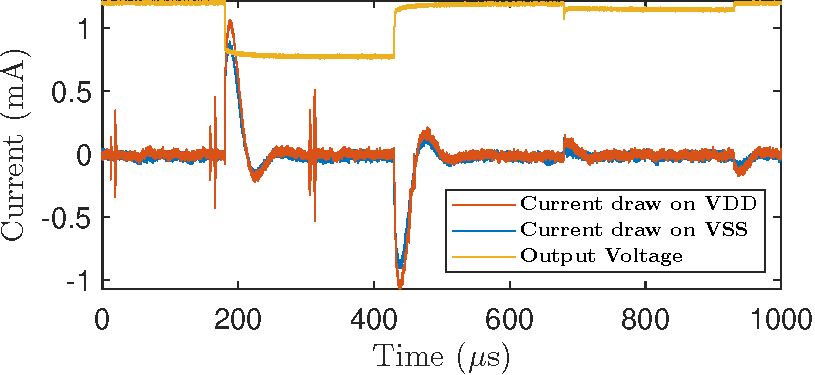
\includegraphics[width=1\linewidth]{Images/NAND2kI.pdf}
    \caption{Plot showing current draw for NAND gate at 2 kHz, the highest of the sampled frequencies that exhibits zero current draw unless the output state is transitioning. The gate output voltage has been scaled and offset to the top of the diagram.}
    \label{fig:I2K}
\end{figure}
\begin{figure}[b]
    \centering
    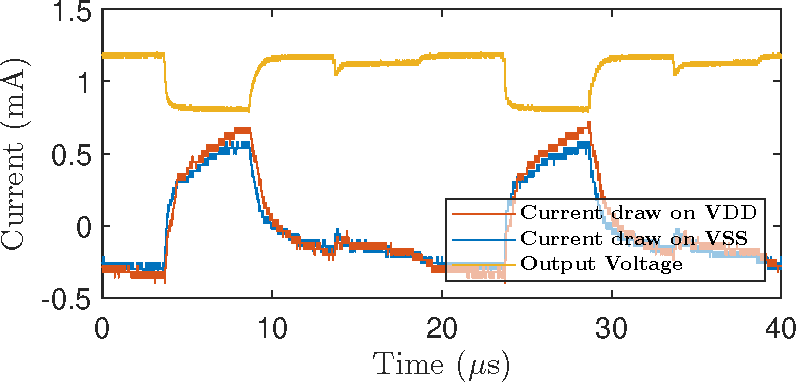
\includegraphics[width=1\linewidth]{Images/NAND100kI.pdf}
    \caption{Plot showing current draw for NAND gate at 100 kHz. This is the operational frequency of the CPU as simulated in this paper and shows that the device will always draw current regardless of input states at these frequencies. The gate output voltage has been scaled and offset to the top of the diagram.}
    \label{fig:I100K}
\end{figure}
\fi

\subsubsection{Floating Point Multiplication Subroutine}
The floating point system implemented takes the following form.
\begin{equation}\label{floatform}
    (-1)^{\text{signbit}} \times 1.sssssss \times 2^{eeeeeee - 63}
\end{equation}
where $s$ denotes a significand bit and $e$ denotes an exponent bit. The processor-level functionality is further demonstrated by the computation $1.4375 \times 3.609375$, which gives $5.1875$ after rounding in the implemented floating-point representation.

The implemented floating-point format rounds the exact product $5.18847\ldots$ to $5.1875$, as shown in Table~\ref{tab:multiplicationvalues}. \ifjxcdc A full description of the algorithm is given in the supplementary material.\else Explanations of the algorithm can be found in Appendix \hyperref[appB]{A}.\fi
\ifjxcdc\else
The final values in the registers in Figures \ref{fig:sig} and \ref{fig:exp} being zero is due to an LTspice simulation error which occurred after the program had finished running.
\fi

\subsection{Experimental Data}
The logic gates were tested at input frequencies from 1\,Hz up to 800\,kHz (NOR) and 1\,MHz (NAND).
\ifjxcdc
Figure~\ref{fig:NAND100K} shows the 100\,kHz operating point at which the CPU is simulated, and Figure~\ref{fig:NOR800k} shows the highest frequency at which the NOR primitive still produced an adequate output swing. Per-frequency NAND and NOR comparisons across the full 1\,Hz--1\,MHz range, including current-draw plots, are given in the supplementary material.
\else
Figures~\ref{fig:NAND100K} and~\ref{fig:NOR100K} show the 100\,kHz operating point at which the CPU is simulated, and Figures~\ref{fig:NAND1000K} and~\ref{fig:NOR800k} show the highest tested frequency for each gate.
\fi
Above 800\,kHz the NOR output swing collapses because the rise time exceeds the half-period, and the gate can no longer respond to its inputs. For the tested two-input primitives, the NOR gate is therefore the measured limiting case, with adequate output swing up to 800\,kHz; the NAND gate continues to switch cleanly to 1\,MHz. Both bounds are comfortably above the 100\,kHz simulated CPU clock.

\begin{table}[H]
\centering
\caption{Floating Point Number Values Used in Subroutine}
\label{tab:multiplicationvalues}
\begin{tabular}{@{}llll@{}}
\toprule
Binary & Decimal & Exponential Form & Value\\ \midrule
10111000 00111111 & 184 63 & $1.4375 \times 2^0$ & 1.4375\\
11100111 01000000 & 231 64 & $1.8046875 \times 2^1$ & 3.609375\\
10100110 01000001 & 166 65 & $1.296875 \times 2^2$ & 5.1875\\\bottomrule
\end{tabular}
\end{table}

\ifjxcdc\else
\begin{table}[H]
\centering
\caption{Register values for Figures \ref{fig:sig} and \ref{fig:exp}}
\label{tab:fig16and17values}
\begin{tabular}{@{}llll@{}}
\toprule
Clock Cycle & Significand & Exponent & Decimal\\ \midrule
0    & 255 & 255 & $1.9921875 \times -2^{64}$\\
370  & 0   & 255 & $0$\\
828  & 0   & 127 & $0$\\
924  & 0   & 112 & $0$\\
1020 & 0   & 64  & $0$\\
1527 & 184 & 64  & $2.875$\\
2178 & 40  & 64  & $0.625$\\
2830 & 8   & 64  & $0.125$\\
6580 & 4   & 64  & $0.0625$\\
6968 & 130 & 64  & $2.03125$\\
7356 & 193 & 64  & $3.015625$\\
7744 & 96  & 64  & $1.5$\\
8128 & 48  & 64  & $0.75$\\
8608 & 152 & 64  & $2.375$\\
9039 & 76  & 64  & $1.1875$\\
9472 & 166 & 64  & $2.59375$\\
9640 & 166 & 65  & $5.1875$\\ \bottomrule
\end{tabular}
\end{table}
\fi

The primitive-gate measurements show that the measured SiC JFET RTL gates switch comfortably above the 100\,kHz CPU simulation clock; this should not be read as a measured full-processor $f_{\max}$, since the complete CPU was not fabricated and the critical paths are only evaluated in LTspice. For reference, the original Intel 4004 silicon was specified at $\sim$740\,kHz peak, with the commonly quoted 400\,kHz referring to the typical operating frequency rather than the maximum.

\begin{figure}[b]
    \centering
    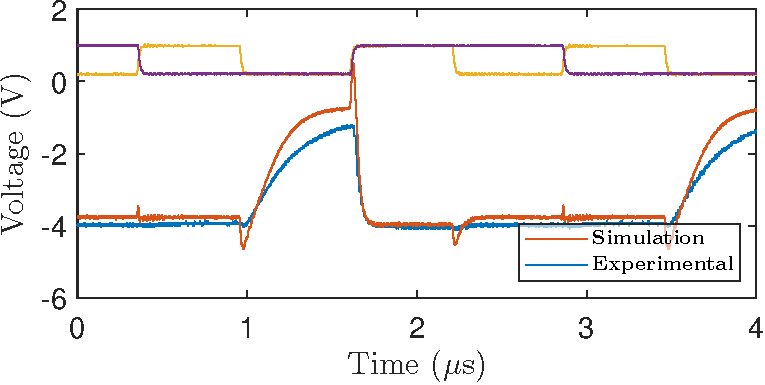
\includegraphics[width=\linewidth]{Images/NOR800K.pdf}
    \caption{Experimental and simulation output voltages of a NOR gate at 800\,kHz, the maximum frequency at which the NOR gate produced adequate output peaks. Inputs scaled and offset as before. Raw oscilloscope traces are not retained; the 1.5--2\,V baseline shift is discussed in Section~\ref{sec:limitations}.}
    \label{fig:NOR800k}
\end{figure}

\ifjxcdc\else
\begin{figure}[t]
    \centering
    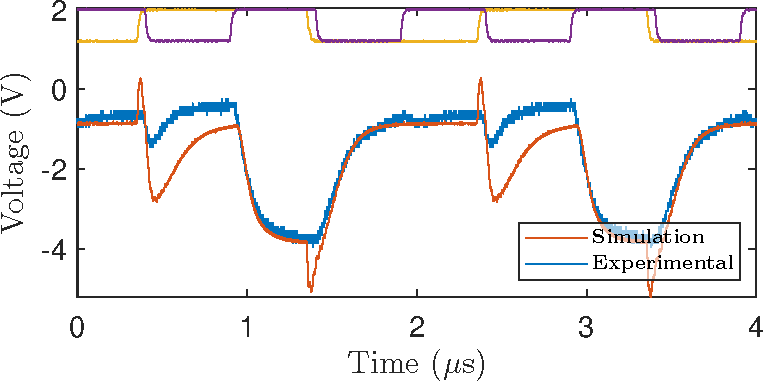
\includegraphics[width=\linewidth]{Images/NAND1000K.pdf}
    \caption{Experimental and simulation output voltages of a NAND gate at 1\,MHz, the maximum frequency at which the NAND gate was tested. Inputs scaled and offset as before. Raw oscilloscope traces are not retained; the baseline shift, which grows with frequency for the NAND gate, is discussed in Section~\ref{sec:limitations}.}
    \label{fig:NAND1000K}
\end{figure}
\fi

The oscilloscope probes introduced scaling by a factor of two, necessitating post-experimental adjustments. There was a 1.5 - 2 V baseline shift in the data compared to what was expected from the simulations, the origins of which are currently under investigation. Some of the difference was due to resistor inaccuracies, however, this cannot account for the entire 2 V shift. Further, it can be seen that as the frequency increases this offset increases, starting at approximately 1.5 V at 2 Hz going up to approximately 2 V at 100 kHz. This indicates that it is some function of the JFETs themselves. This change in output voltage levels as a function of frequency was only observed in the NAND gate. The NOR gate retained its 1.5 V shift for the entire range of examined frequencies. This could be due to differences in the JFETs used between the NAND and NOR gates rather than due to gate topology. Further investigation into the nature of these discrepancies is necessary to determine their source, be it manufacturing variability or the LTspice model itself. The voltage levels and resistor values used should be explored in greater depth to determine optimum performance for specific applications.

\ifjxcdc\else
The current draw demonstrated by the NAND gate at lower frequencies displays CMOS like qualities where it is only actively drawing current on the transition between output states as shown in Figure \ref{fig:I2K}. This behaviour was not apparent at higher frequencies as shown in Figure \ref{fig:I100K}. This is an unexpected result and should be investigated further. The current draw on each voltage source (positive supply voltage: 24 V, negative supply voltage: -20 V) was about 0.5 mA per logic gate which consisted of 3 transistors. Extrapolating from this, the peak current draw for the full CPU of \TotalJFETCount{} transistors would be of order 900\,mA. Due to the CMOS like nature of the current draw at lower frequencies, if entire systems of the CPU such as the lower levels of the stack or some scratchpad registers are not being used, the current draw would be lower.
\fi

\section{Limitations}\label{sec:limitations}

Three classes of limitation deserve explicit acknowledgement.

\textit{Measured primitive gates exhibit a 1.5--2\,V baseline offset relative to the simulated waveforms} (\ifjxcdc Figures \ref{fig:NAND100K}, \ref{fig:NOR800k}\else Figures \ref{fig:NAND100K}, \ref{fig:NOR100K}, \ref{fig:NOR800k}, \ref{fig:NAND1000K}\fi). The offset is approximately constant for the NOR gate across the entire measured frequency range, and grows mildly with frequency for the NAND. Resistor tolerance is too small to account for the magnitude; this points instead either to manufacturing variability of the SiC JFET die used (a single integrated circuit was the source of devices for both gates) or to a residual modelling gap in the JFET parameter card used for the LTspice simulation. The waveform \emph{shape} (transitions, settling, and frequency response) matches the simulation closely over 1\,Hz to 800\,kHz for the NOR and 1\,Hz to 1\,MHz for the NAND, which is the basis on which the simulated CPU is asserted to be functionally representative; the absolute offset is an open discrepancy and should not be read as a confirmation of the simulation's quantitative voltage levels.

\textit{The full processor is not fabricated.} All system-level claims rest on LTspice transient simulation of the complete \TotalJFETCount{}-transistor design, cross-validated against an independent Python reference emulator at every instruction boundary (Section~\ref{method}). The strongest experimental evidence in this paper is for the primitive gates only. A fabricated CPU is the obvious next step, but the dominant transistor budget --- D flip-flop storage rather than combinational logic --- would benefit substantially from a single-transistor DRAM cell before fabrication is attempted.

\textit{The LTspice device model used is at room temperature.} The CPU simulations use a SiC JFET parameterisation supplied for this project, evaluated at 27\,\degree C; high-temperature behaviour is by extrapolation only. The parameter card itself appeared in the publicly released MEng report from which this work descends and is shipped with the reproducibility package on that basis; the underlying device model belongs to its original owner, and any redistribution beyond academic reproduction should obtain permission accordingly. The radiation-hardness and high-temperature motivation for SiC JFET computing remains; what this work demonstrates is that an Intel-4004-compatible architecture is feasible in a SiC JFET RTL logic family, not that the specific design operates at the temperatures motivating it. A temperature-scaled re-simulation of the worst-case combinational chain and the noise-margin corner sweep is a natural follow-up, deferring the chip-level fabrication question while strengthening the temperature claim.

\textit{A full fanout / noise-margin / critical-path characterisation of the integrated design remains future work.} The 100\,kHz CPU claim rests on LTspice transient execution of the reported test programs rather than on a systematic worst-case critical-path extraction across all 46 instructions, and the primitive-gate frequency results in Section~\ref{sec_results} should not be read as a substitute. The corner-sweep test benches that would produce noise-margin and timing tables -- under $\pm 20\%$ resistor variation and $\pm 2$\,V supply variation -- are included in the reproducibility package (\texttt{analysis/sweeps/}) but not yet executed; the corresponding result tables will be added in revision.

\section{Conclusion}\label{conclusion}

This paper has presented a transistor-level SiC JFET implementation of an Intel-4004-compatible 4-bit microprocessor, comprising \TotalJFETCount{} JFETs (Table~\ref{tab:transistor-count}) across the ALU, instruction register and decoder, program counter, three-level stack, and sixteen-register scratch pad; a compatible 4001-style ROM model is used for program execution and is not included in this JFET count. The simulated CPU design is supported by two independent forms of evidence: register-level program co-validation against a Python reference emulator at every instruction boundary, demonstrated on a 30-byte bitwise AND subroutine and a 16-bit floating-point multiplication producing a 451-instruction execution trace; and measured waveform-shape and switching-frequency consistency of NAND and NOR primitives built from a discrete SiC JFET integrated circuit, characterised from 1\,Hz to 800\,kHz (NOR) and 1\,MHz (NAND).

The largest practical constraint on further work is the storage cost of D flip-flops: 146 bits of scratch-pad and stack storage account for 2190 JFETs of the \TotalJFETCount{} total. The design therefore remains substantially larger than the original NMOS 4004, primarily because the present storage implementation uses 15-JFET D flip-flops rather than 1T DRAM cells. A SiC JFET DRAM cell would close most of this gap. The remaining open discrepancy in this paper --- the 1.5--2\,V baseline offset between measured and simulated primitive gates --- is a candidate next investigation, and is most cheaply pursued by repeating the NAND/NOR measurement with multiple device samples to separate manufacturing variability from a residual modelling gap. A temperature-scaled re-simulation of the worst-case combinational chain and the noise-margin corner sweep is a complementary follow-up that strengthens the high-temperature claim without requiring fabrication. The fabrication of the full 4004-compatible processor in SiC JFET is the eventual target; the work presented here establishes that a complete architecture-scale design and a validation methodology now exist to support that step.
\section*{Acknowledgements}
This work originated as an MEng research project at Durham University. The authors thank the Department of Engineering for access to test equipment, and the maintainers of LTspice for making the simulator freely available.
\printbibliography
\ifjxcdc
% Appendices are omitted from the JXCDC compressed variant. The full
% MCS-4 bitwise AND assembly listing, the floating-point multiplication
% algorithm description, and the expanded register-trace plots are
% provided in the supplementary material that accompanies this paper.
\else
\begin{appendices}
\newpage
\section*{Appendix A}
\label{appB}
\begin{figure}[H]
\begin{lstlisting}[
language={[x86masm]Assembler},
caption={Assembly Code for SIGNBITS function},
label=SIGNBITS
]
SIGNBITS CLC
LD 6
RAL
TCC
XCH 2
LD 6
RAL
CLC
RAR
XCH 6
CLC
LD 10
RAL
TCC
XCH 3
LD 10
RAL
CLC
RAR
XCH 10
BBL 0
\end{lstlisting}
\end{figure}

\begin{figure}[H]
\begin{lstlisting}[
language={[x86masm]Assembler},
caption={Assembly Code for initialising registers for multiplication function},
label=Init
]
START LDM 15
XCH 4
LDM 4
XCH 5
LDM 4
XCH 6
LDM 7
XCH 7
LDM 10
XCH 8
LDM 0
XCH 9
LDM 4
XCH 10
LDM 11
XCH 11
JMS MULT
NOP
\end{lstlisting}
\end{figure}

The way the multiplication algorithm (Listing \ref{MultRoutine}) works is two separate computations. First the sign bit is extracted from the exponent using the SIGNBITS Subroutine (Listing \ref{SIGNBITS}). Then the two exponents are added together, however this means that the offset of 63 has been added twice and needs to be subtracted to get the final value. Next the significands need to be multiplied. This is achieved by checking the lowest order bit of the multiplier. If it is high, the multiplicand is added to the output register, the multiplicand is shifted to the left and the multiplier is shifted to the right. This then repeats until the entire multiplier has been checked and the final answer can be read. There are some tricks that have been done to preserve accuracy of the final answer such as using 4 registers to store the multiplicand and the product allowing for 16 bits of accuracy. The final step shifts the entire product until it detects that there are no 1s in the two registers used for the highest order bits. If the product is shifted more than 8 times it indicates that the product required normalising, shifting so that there is a 1 in the highest order bit. If this occurs, 1 needs to be added to the exponent for each time the product is shifted past 8 times.

\begin{figure}[h]
\begin{lstlisting}[
language={[x86masm]Assembler},
caption={Assembly Code for floating point multiplication subroutine},
label=MultRoutine,
basicstyle=\ttfamily\scalefont{0.62}
]
MULT FIM 6 0 0
JMS SIGNBITS
LD 7
ADD 11
XCH 15
LD 6
ADD 10
XCH 14
CLC
LDM 15
XCH 0
LD 15
SUB 0
XCH 15
CMC
LDM 3
XCH 0
LD 14
SUB 0
XCH 14
CLC
LD 2
ADD 3
RAL
RAL
RAL
CLC
ADD 14
XCH 14
FIM 0 0 0
FIM 1 0 0
BCHECK LD 8
JCN 12 IF1
LD 9
JCN 12 IF1
JUN RETURN
IF1 CLC
LD 8
RAR
XCH 8
LD 9
RAR
XCH 9
JCN 10 IF2
CLC
LD 13
ADD 5
XCH 13
LD 12
ADD 4
XCH 12
LD 3
ADD 1
XCH 3
LD 2
ADD 0
XCH 2
IF2 CLC
LD 5
RAL
XCH 5
LD 4
RAL
XCH 4
RAL
LD 1
RAL
XCH 1
LD 0
RAL
XCH 0
JUN BCHECK
RETURN LD 2
JCN 12 IF3
LD 3
JCN 12 IF3
JUN MULTEND
IF3 LD 2
RAR
XCH 2
LD 3
RAR
XCH 3
LD 12
RAR
XCH 12
LD 13
RAR
XCH 13
CLC
JUN RETURN
MULTEND BBL 0
\end{lstlisting}
\end{figure}

\clearpage
\newpage
\section*{\centering Appendix B}
\label{appC}
\begin{figure}[H]
\begin{lstlisting}[
language={[x86masm]Assembler},
caption={Assembly Code for AND Subroutine},
label=ANDRoutine
]
JUN START
AND FIM 1 0 11
Loop LDM 0
XCH 0
RAL
XCH 0
INC 3
XCH 3
JCN 4 Done
XCH 3
RAR
XCH 2
XCH 1
RAL
XCH 1
RAR
ADD 2
JUN Loop
Done BBL 0
START LDM 11
XCH 0
LDM 6
XCH 1
JMS AND
NOP
\end{lstlisting}
\end{figure}

The AND subroutine produces the AND of two input words by placing the bits in the leftmost position of the accumulator \ref{ACC} and register 2 \ref{Scratch2}, respectively, and zeroing the rightmost three bits of the accumulator and register 2. Register 2 is then added to the accumulator, and the resulting carry is equal to the AND of the two bits. Scratch Pad register 3 (Figure \ref{Scratch3}) is used as the counter, counting up from 11. When this overflows from 15 to 0 the program breaks and returns.

\begin{figure*}[h]
\centering
\subcaptionbox{Scratchpad 0 value, containing the first input word which is shifted left four times. This is the register the function returns the output value to. The shifts are as follows, 1011 to 0110 to 1100 to 1000. The returned value is then placed in and shifted once, 0001 to 0010.\label{Scratch0}}
{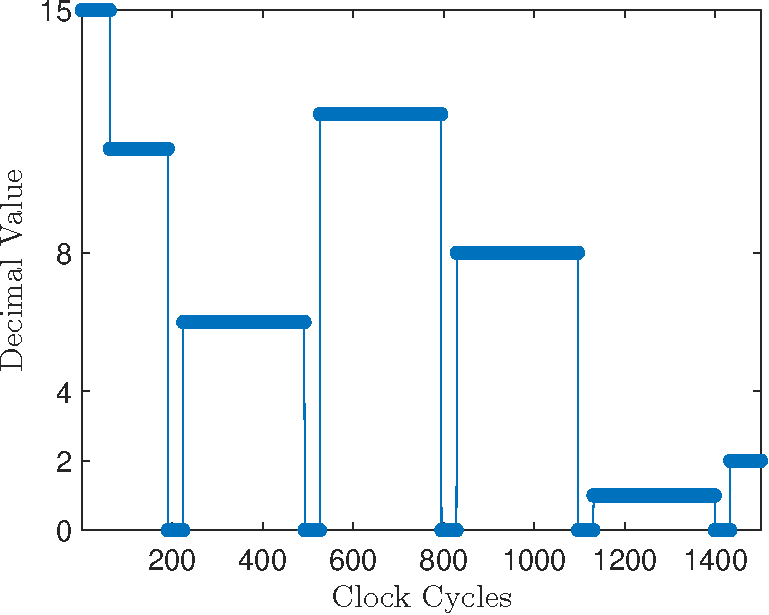
\includegraphics[width=0.49\linewidth, height = 0.2\textheight]{Appendices/Scratchpad0.pdf}}
\subcaptionbox{Scratchpad 1 value, containing the second input word which is shifted left three times. The shifts are as follows, 0110 to 1100 to 1000 to 0000.\label{Scratch1}}
{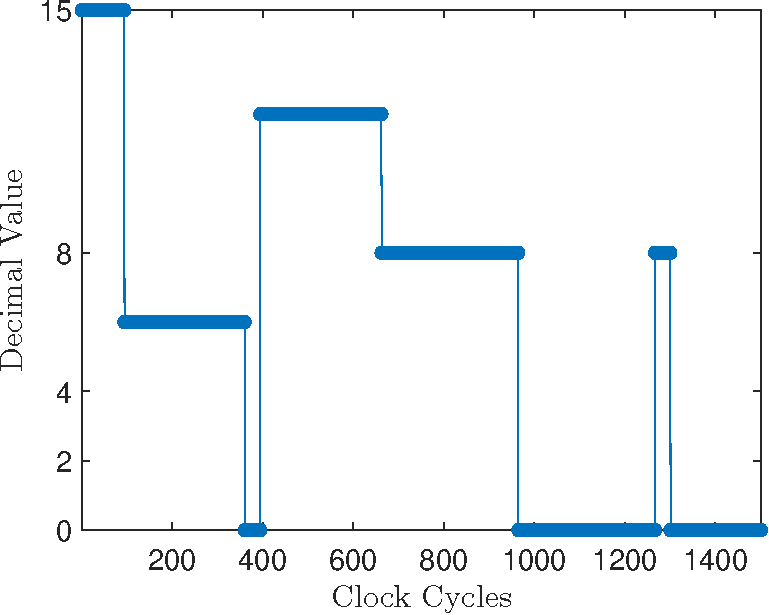
\includegraphics[width=0.49\linewidth, height = 0.2\textheight]{Appendices/Scratchpad1.pdf}}
\caption{Scratchpad Pair 0, the input and output registers.\label{Scratch00}}
\end{figure*}

\begin{figure*}[h]
\centering
\subcaptionbox{Scratchpad 2 value, this is working memory for the program. The highest order bit from one input is put into here and added to the accumulator which contains the high order bit from the other input.\label{Scratch2}}
{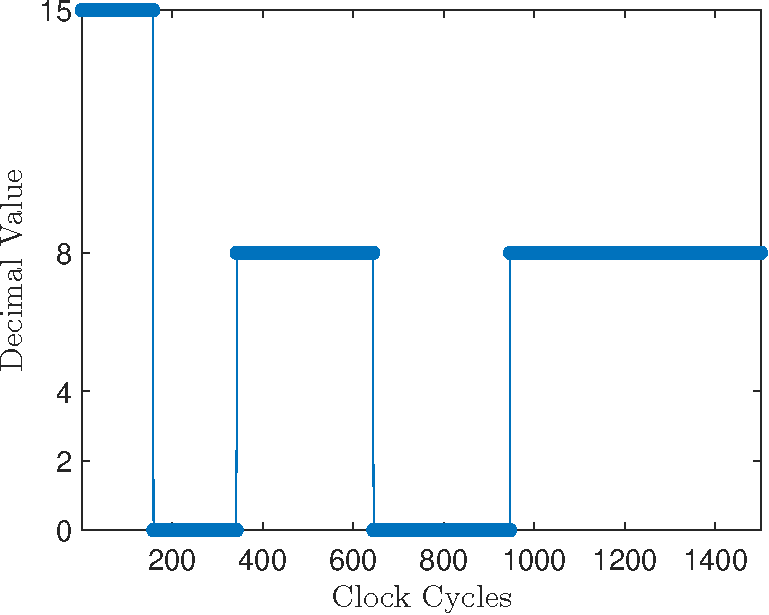
\includegraphics[width=0.49\linewidth, height = 0.2\textheight]{Appendices/Scratchpad2.pdf}}
\subcaptionbox{Scratchpad 3 value, this is the counter for counting the number of times register 0 has been shifted. This starts at 11 and the program breaks when the value overflows from 15 to 0.\label{Scratch3}}
{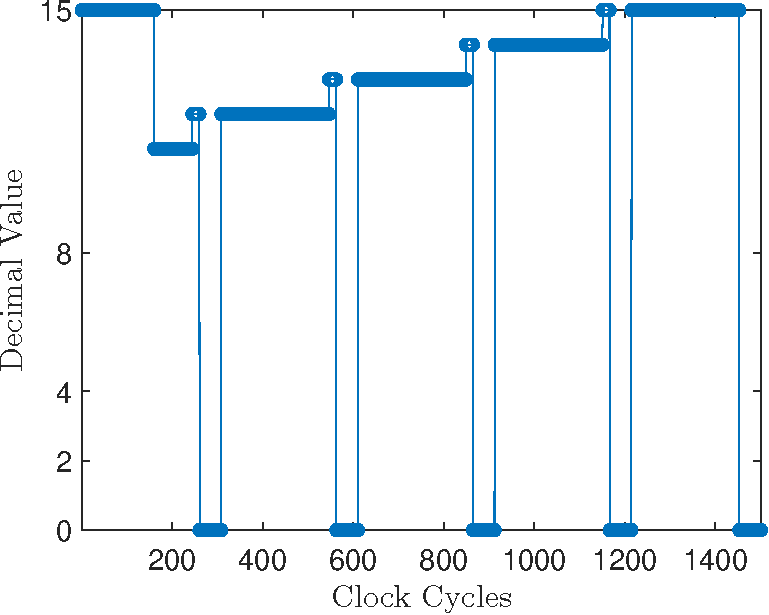
\includegraphics[width=0.49\linewidth, height = 0.2\textheight]{Appendices/Scratchpad3.pdf}}
\caption{Scratchpad Pair 1\label{Scratch01}}
\end{figure*}

\begin{figure*}[h]
\centering
\subcaptionbox{Accumulator register value\label{ACC}}
{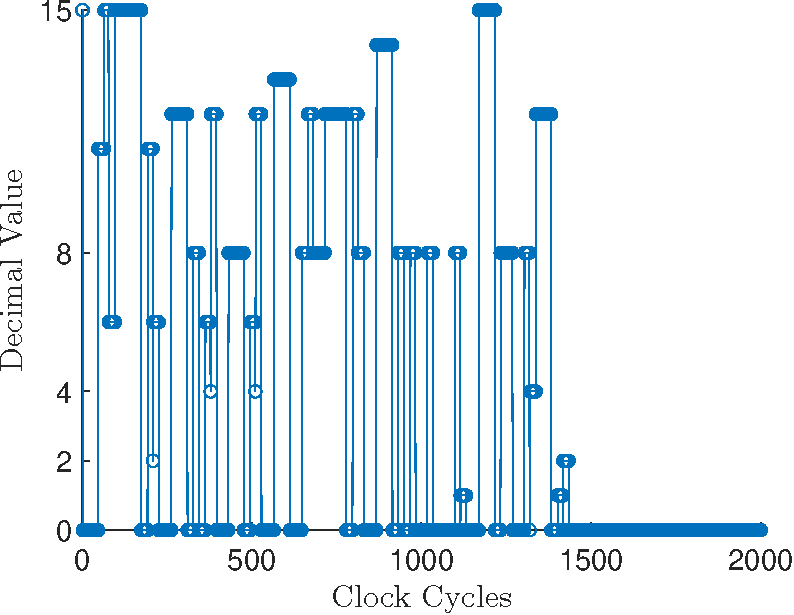
\includegraphics[width=0.49\linewidth, height = 0.2\textheight]{Appendices/ACC.pdf}}
\subcaptionbox{Carry Flag register value, when the highest bit of word one and word two are added together the carry is equal to the AND of the two bits\label{CF}}
{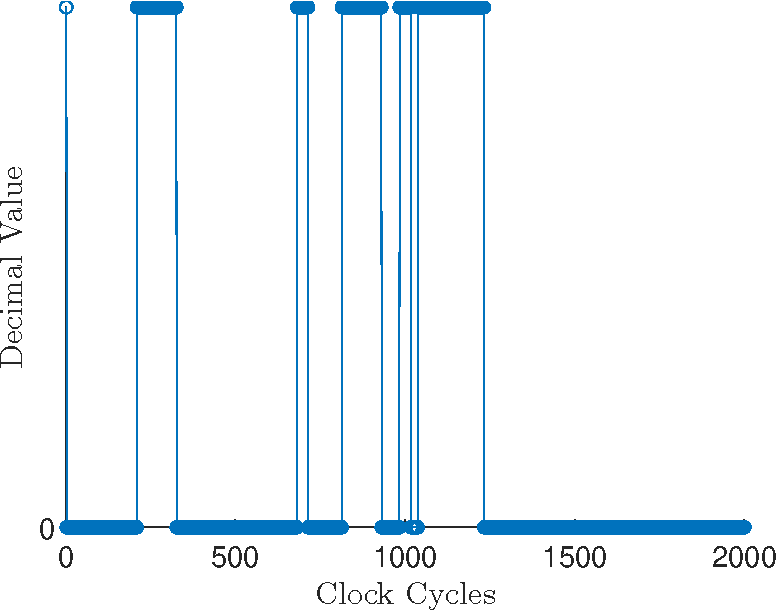
\includegraphics[width=0.49\linewidth, height = 0.2\textheight]{Appendices/CF.pdf}}
\caption{Accumulator and Carry Flag register values\label{ACCCF}}
\end{figure*}


\end{appendices}
\fi
